\documentclass{article}
\usepackage{fullpage,graphicx}
\usepackage{hyperref}
\usepackage[
  backend=bibtex,
  style=numeric,
  maxcitenames=2]{biblatex}
\addbibresource{ref}
\def\sectionautorefname{Section}
\def\subsectionautorefname{Subsection}
\def\subsubsectionautorefname{Subsubsection}
\def\lstnumberautorefname{Line}
\usepackage[dvipsnames,svgnames,x11names]{xcolor}
\usepackage{textcomp,listings,lstparams,lstcoq,xspace}
\lstdefinestyle{customcoq}{
  language=Coq,
  literate={<>}{$\ne$}1
  {->}{$\to$}1
}
\lstdefinestyle{json}{
  language=Coq,
  literate={@}{$@$}1
  {this}{$\ottkw{this}$}4
  {ref}{$\ottkw{ref}$}3
}
\lstdefinestyle{customc}{
  language=C
}
\newcommand{\http}{HTTP/1.1\xspace}
\newcommand{\inlinec}[1]{\lstinline[style=customc]{#1}}
\newcommand{\ilc}[1]{\lstinline[style=customcoq]{#1}}
\newcommand{\ilj}[1]{\lstinline[style=json]{#1}}

\usepackage{draft} % local
\newif\ifdraft\drafttrue
\newnote{lys}{BrickRed}
\newnote{bcp}{Chocolate}
\newnote{sz}{violet}

\usepackage{amsthm,amssymb}
\theoremstyle{definition}
\newtheorem{definition}{Definition}

\newcommand{\Nat}{\mathbb N}
\newcommand{\Let}{\ottkw{let}\;}
\newcommand{\In}{\;\ottkw{in}}
\newcommand{\letin}[2]{\Let#1=#2\In}
\newcommand{\sigT}[2]{\{\exists#1,#2\}}
\newcommand{\existT}[3]{\ottkw{pack}\;#1=#2\;\ottkw{with}\;#3}
\newcommand{\Server}{\ottkw{Server}}
\newcommand{\Validator}{\ottkw{Validator}}
\newcommand{\stepServer}{\ottkw{stepServer}}
\newcommand{\stepValidator}{\ottkw{stepValidator}}
\newcommand{\sstep}{\ottkw{sstep}}
\newcommand{\vstep}{\ottkw{vstep}}
\newcommand{\option}{\ottkw{option}\;}
\newcommand{\Some}[1]{\ottkw{Some}\;#1}
\newcommand{\None}{\varnothing}
\newcommand{\List}{\ottkw{list}\;}
\newcommand{\nil}{\varepsilon}
\newcommand{\yields}[3]{#1\overset{#2}{\longrightarrow}#3}
\newcommand{\accepts}[3]{#1\overset{#2}{\longrightarrow}#3}
\newcommand{\sound}{\ottkw{sound}}
\newcommand{\issound}[2]{#1\;\sound_{#2}}
\newcommand{\complete}{\ottkw{complete}}
\newcommand{\iscomplete}[2]{#1\;\complete_{#2}}
\newcommand{\Prog}{\ottkw{Prog}}
\newcommand{\serverOf}{\ottkw{serverOf}}
\newcommand{\validatorOf}{\ottkw{validatorOf}}
\newcommand{\Reflects}[2]{#1\sim #2}
\newcommand{\Constraint}{\ottkw{Constraint}}
\newcommand{\fresh}{\ottkw{fresh}}
\newcommand{\solvable}{\ottkw{solvable}}
\newcommand{\Write}{\ottkw{write}}
\newcommand{\Havoc}{\ottkw{havoc}}
\newcommand{\Exec}{\ottkw{exec}}
\newcommand{\If}{\ottkw{if}\;}
\newcommand{\Then}{\ottkw{then}\;}
\newcommand{\Else}{\ottkw{else}\;}
\newcommand{\bool}{\mathbb B}
\newcommand{\Assignment}{\ottkw{Assignment}}
\newcommand{\Evaluate}{\ottkw{evaluate}}
\newcommand{\Satisfy}{\ottkw{satisfy}}
\newcommand{\true}{\ottkw{true}}
\newcommand{\false}{\ottkw{false}}
\newcommand{\imp}{\ottkw{implements}}
\newcommand{\pass}{\ottkw{passes}}
\newcommand{\exhaust}{\ottkw{exhaustive}}
\newcommand{\defeq}{\triangleq}
\newcommand{\implements}[2]{#1\;\imp\;#2}
\newcommand{\passes}[2]{#1\;\pass\;#2}
\newcommand{\isexhaust}[1]{#1\;\exhaust}

% generated by Ott 0.31 from: jexp.ott
\usepackage{amsmath,amssymb}
\usepackage{supertabular}
\usepackage{geometry}
\usepackage{ifthen}
\usepackage{alltt}%hack
\geometry{a4paper,dvips,twoside,left=22.5mm,right=22.5mm,top=20mm,bottom=30mm}
\usepackage{color}
\newcommand{\ottdrule}[4][]{{\displaystyle\frac{\begin{array}{l}#2\end{array}}{#3}\quad\ottdrulename{#4}}}
\newcommand{\ottusedrule}[1]{\[#1\]}
\newcommand{\ottpremise}[1]{ #1 \\}
\newenvironment{ottdefnblock}[3][]{ \framebox{\mbox{#2}} \quad #3 \\[0pt]}{}
\newenvironment{ottfundefnblock}[3][]{ \framebox{\mbox{#2}} \quad #3 \\[0pt]\begin{displaymath}\begin{array}{l}}{\end{array}\end{displaymath}}
\newcommand{\ottfunclause}[2]{ #1 \equiv #2 \\}
\newcommand{\ottnt}[1]{\mathit{#1}}
\newcommand{\ottmv}[1]{\mathit{#1}}
\newcommand{\ottkw}[1]{\mathbf{#1}}
\newcommand{\ottsym}[1]{#1}
\newcommand{\ottcom}[1]{\text{#1}}
\newcommand{\ottdrulename}[1]{\textsc{#1}}
\newcommand{\ottcomplu}[5]{\overline{#1}^{\,#2\in #3 #4 #5}}
\newcommand{\ottcompu}[3]{\overline{#1}^{\,#2<#3}}
\newcommand{\ottcomp}[2]{\overline{#1}^{\,#2}}
\newcommand{\ottgrammartabular}[1]{\begin{supertabular}{llcllllll}#1\end{supertabular}}
\newcommand{\ottmetavartabular}[1]{\begin{supertabular}{ll}#1\end{supertabular}}
\newcommand{\ottrulehead}[3]{$#1$ & & $#2$ & & & \multicolumn{2}{l}{#3}}
\newcommand{\ottprodline}[6]{& & $#1$ & $#2$ & $#3 #4$ & $#5$ & $#6$}
\newcommand{\ottfirstprodline}[6]{\ottprodline{#1}{#2}{#3}{#4}{#5}{#6}}
\newcommand{\ottlongprodline}[2]{& & $#1$ & \multicolumn{4}{l}{$#2$}}
\newcommand{\ottfirstlongprodline}[2]{\ottlongprodline{#1}{#2}}
\newcommand{\ottbindspecprodline}[6]{\ottprodline{#1}{#2}{#3}{#4}{#5}{#6}}
\newcommand{\ottprodnewline}{\\}
\newcommand{\ottinterrule}{\\[5.0mm]}
\newcommand{\ottafterlastrule}{\\}
\newcommand{\ottmetavars}{
\ottmetavartabular{
 $ \ottmv{l} $ & \ottcom{trace labels} \\
 $ \ottmv{f} $ & \ottcom{functions} \\
 $ \ottmv{s} $ & \ottcom{string literals} \\
 $ \ottmv{i} $ & \ottcom{integers} \\
}}

\newcommand{\ottjexp}{
\ottrulehead{\ottnt{jexp}}{::=}{\ottcom{J-expressions}}\ottprodnewline
\ottfirstprodline{|}{\ottkw{ref} \, \ottmv{l} \, \ottnt{p} \, \ottmv{f}}{}{}{}{}\ottprodnewline
\ottprodline{|}{\ottsym{\{}  \ottnt{object}  \ottsym{\}}}{}{}{}{}\ottprodnewline
\ottprodline{|}{\ottsym{[}  \ottnt{array}  \ottsym{]}}{}{}{}{}\ottprodnewline
\ottprodline{|}{\ottmv{s}}{}{}{}{}\ottprodnewline
\ottprodline{|}{\ottmv{i}}{}{}{}{}\ottprodnewline
\ottprodline{|}{\ottkw{true}}{}{}{}{}\ottprodnewline
\ottprodline{|}{\ottkw{false}}{}{}{}{}\ottprodnewline
\ottprodline{|}{\ottkw{null}}{}{}{}{}}

\newcommand{\ottobject}{
\ottrulehead{\ottnt{object}}{::=}{}\ottprodnewline
\ottfirstprodline{|}{}{}{}{}{}\ottprodnewline
\ottprodline{|}{\ottsym{"}  \ottmv{s}  \ottsym{"}  \ottsym{:}  \ottnt{jexp}  \ottsym{,}  \ottnt{object}}{}{}{}{}}

\newcommand{\ottarray}{
\ottrulehead{\ottnt{array}}{::=}{}\ottprodnewline
\ottfirstprodline{|}{}{}{}{}{}\ottprodnewline
\ottprodline{|}{\ottnt{jexp}  \ottsym{,}  \ottnt{array}}{}{}{}{}}

\newcommand{\ottp}{
\ottrulehead{\ottnt{p}}{::=}{\ottcom{J-paths}}\ottprodnewline
\ottfirstprodline{|}{\ottkw{this}}{}{}{}{}\ottprodnewline
\ottprodline{|}{\ottnt{p}  \ottsym{\#}  \ottmv{i}}{}{}{}{}\ottprodnewline
\ottprodline{|}{\ottnt{p}  \ottsym{@}  \ottmv{s}}{}{}{}{}}

\newcommand{\ottgrammar}{\ottgrammartabular{
\ottjexp\ottinterrule
\ottobject\ottinterrule
\ottarray\ottinterrule
\ottp\ottafterlastrule
}}

% defnss
\newcommand{\ottdefnss}{
}

\newcommand{\ottall}{\ottmetavars\\[0pt]
\ottgrammar\\[5.0mm]
\ottdefnss}



\title{Language Design for Asynchronous Test\\
  \large \medskip Thesis Proposal}
\author{Yishuai Li}
\begin{document}
\maketitle
\section{Introduction}
\label{sec:intro}

The security and robustness of networked systems rest in large part on the
correct behavior of various sorts of servers.  This can be validated either by
full-blown verification or model checking against formal specifications, or
less expensively by rigorous testing.

Rigorous testing requires a rigorous specification of the protocol that we
expect the server to obey.  Protocol specifications can be written as (i) a {\em
  server model} that describes {\em how} valid servers should handle messages,
or (ii) a {\em property} that defines {\em what} server behaviors are valid.
From these specifications, we can conduct (i) {\em model-based
  testing}~\cite{broy2005model} or (ii) {\em property-based testing}~\cite{pbt},
respectively.

When testing server implementations against protocol specifications, one
critical challenge is {\em nondeterminism}, which arises in two forms---we call
them (1) {\em internal nondeterminism} and (2) {\em network nondeterminism}:

(1) {\em Within} the server, correct behavior may be \mbox{underspecified}.
For example, to handle HTTP conditional requests \cite{rfc7232}, a server
generates strings called entity tags (ETags), but the RFC specification does
not limit {what} values these ETags should be.  Thus, to create test
messages containing ETags, the tester must remember and reuse the ETags it
has been given in previous messages from the server.

(2) {\em Beyond} the server, messages and responses between the server and
different clients might be delayed and reordered by the network and
operating-system buffering.  If the tester cannot control how the execution
environment reorders messages---{\it e.g.,} when testing over the Internet---it
needs to specify what servers are valid as observed over the network.

These sources of nondeterminism pose challenges in various aspects of testing network
protocols: (i) The {\em validation logic} should accept various implementations,
as long as the behavior is included in the specification's space of
uncertainties; (ii) To capture bugs effectively, the {\em test harness} should
generate test cases based on runtime observations; (iii) When {\em shrinking} a
counterexample, the test harness should adjust the test cases based on the
server's behavior, which might vary from one execution to another.

To address these challenges, I introduce symbolic languages for writing
specifications and representing test cases:

(i) The specification is written as a reference implementation---a
nondeterministic program that exhibits all possible behavior allowed by
the protocol.  Inter-implementation and inter-execution uncertainties are
represented by symbolic variables, and the space of nondeterministic behavior is
defined by all possible assignments of the variables.

The validation logic is derived from the reference implementation, by {\em
  dualising} the server-side program into a client-side observer.

(ii) Test generation heuristics are defined as computations from the observed
trace (list of sent and received messages) to the next message to send.  I
introduce a symbolic intermediate representation for specifying the relation
between the next message and previous messages.

(iii) The symbolic language for generating test cases also enables effective
shrinking of test cases.  The test harness minimizes the counterexample by
shrinking its symbolic representation.  When running the test with a shrunk
input, the symbolic representations can be re-instantiated into request messages
that reflect the original heuristics.

\paragraph{Thesis claim}
Symbolic abstract representation can address challenges in testing networked systems with uncertain behavior.
Specifying protocols with symbolic reference implementation enables validating
the system's behavior systematically.  Representing test input as abstract
messages allows generating and shrinking interesting test cases.  Combining
these methods result in a rigorous tester that can capture protocol violations
effectively.

\bigskip This claim will be supported by the following publications:
\begin{enumerate}
\item {\it From C to Interaction Trees: Specifying, Verifying, and Testing a
  Networked Server}~\cite{cpp19}, with Nicolas Koh, Yao Li, Li-yao Xia, Lennart
  Beringer, Wolf Honor\'e, and William Mansky, where I developed a tester
  program based on the swap server's ITree specification, and evaluated the
  tester's effectiveness by mutation testing.
\item {\it Verifying an HTTP Key-Value Server with Interaction Trees and
  VST}~\cite{itp21}, with Hengchu Zhang, Wolf Honor\'e, Nicolas Koh, Yao Li,
  Li-yao Xia, Lennart Beringer, and William Mansky, where I developed the
  top-level specification for \http, and derived a tester client that revealed
  liveness and interrupt-handling bugs in our HTTP server, despite it was
  formally verified.
\item {\it Model-Based Testing of Networked Applications}~\cite{issta21}, which
  describes my technique of specifying \http with symbolic reference
  implementations, and from the specification, automatically deriving a tester
  program that can find bugs in Apache and Nginx.
\item A theory for model-based asynchronous testing, explaining how to specify
  protocols using abstract model implementations, and how to guarantee the
  soundness and completeness of the validator logic derived from the abstract
  model.
\item An experience report on test harness design, introducing an intermediate
  representation for specifying test input generation heuristics, and a generic
  framework for running the tests and shrinking the counterexamples.
\end{enumerate}

This proposal is structured as follows: \autoref{sec:challenges} describes the
challenges caused by internal and network nondeterminism.
\autoref{sec:related-work} lists related works in testing network protocols.
\autoref{sec:practices} and \ref{sec:previous-theories} introduce my previous
experiments and developed theories.  \autoref{sec:research-plan} and
\ref{sec:criteria} discuss my plan towards finishing this thesis, with technical
details in \autoref{sec:appendix-ir}.

\section{Challenges}
\label{sec:challenges}
The Deep Specification project~\cite{deepspec} aims at building a web server and
guarantee its functional correctness with respect to formal specification of the
network protocol.

\http requests can be conditional: if the client has a local copy of some
resource and the copy on the server has not changed, then the server needn't
resend the resource.  To achieve this, an \http server may generate a short
string, called an ``entity tag'' (ETag), identifying the content of some
resource, and send it to the client:
\begin{lstlisting}[style=customc]
/* Client: */
GET /target HTTP/1.1

/* Server: */
HTTP/1.1 200 OK
ETag: "tag-foo"
... content of /target ...
\end{lstlisting}
The next time the client requests the same resource, it can include the ETag in
the GET request, informing the server not to send the content if its ETag still
matches:

\begin{lstlisting}[style=customc]
/* Client: */
GET /target HTTP/1.1
If-None-Match: "tag-foo"

/* Server: */
HTTP/1.1 304 Not Modified
\end{lstlisting}

If the tag does not match, the server responds with code 200 and the updated
content as usual.  Similarly, if a client wants to modify the server's resource
atomically by compare-and-swap, it can include the ETag in the PUT request as
\inlinec{If-Match} precondition, which instructs the server to only update the
content if its current ETag matches.

Thus, whether a server's response should be judged {\em valid} or not
depends on the ETag it generated
when creating the resource.  If the tester doesn't know the server's internal
state ({\it e.g.}, before receiving any 200 response including the ETag), and
cannot enumerate all of them (as ETags can be arbitrary strings), then it needs
to maintain a space of all possible values, narrowing the space upon further
interactions with the server.

\begin{figure}
  \begin{lstlisting}[style=customcoq,mathescape=true]
(* update : (K -> V) * K * V -> (K -> V) *)
let check (trace  : stream http_message,
           data   : key -> value,
           is     : key -> etag,
           is_not : key -> list etag) =
  match trace with
  | PUT(k,t,v) :: SUCCESSFUL :: tr' =>
    if t $\in$ is_not[k] then reject
    else if   is[k] == unknown
            $\vee$ strong_match(is[k],t)
         then let d' = update(data,k,v)     in
              let i' = update(is,k,unknown) in
              let n' = update(is_not,k,[])  in
       (* Now the tester knows that
        * the data in [k] is updated to [v],
        * but its new ETag is unknown. *)
              check(tr',d',i',n')
         else reject
  | PUT(k,t,v) :: PRECONDITION_FAILED :: tr' =>
    if strong_match(is[k],t) then reject
    else let n' = update(is_not, k, t::is_not[k])
      (* Now the tester knows that
       * the ETag of [k] is other than [t]. *)
         in check(tr',data,is,n')
  | GET(k,t) :: NOT_MODIFIED :: tr' =>
    if t $\in$ is_not[k] then reject
    else if is[k] == unknown $\vee$ weak_match(is[k],t)
         then let i' = update(is,k,t) in
       (* Now the tester knows that
        * the ETag of [k] is equal to [t]. *)
              check(tr',data,i',is_not)
         else reject
  | GET(k,t0) :: OK(t,v) :: tr' =>
    if weak_match(is[k],t0) then reject
    else if data[k] $\neq$ unknown $\wedge$ data[k] $\neq$ v
         then reject
         else let d' = update(data,k,v) in
              let i' = update(is,  k,t) in
       (* Now the tester knows
        * the data and ETag of [k]. *)
              check(tr',d',i',is_not)
  | _ :: _ :: _  => reject
  end
  \end{lstlisting}
  \caption{Ad hoc tester for \http conditional requests, demonstrating how
    tricky it is to write the logic by hand.  The checker determines whether a
    one-client-at-a-time \ilc{trace} is valid or not.  The trace is represented
    as a stream (infinite linked list, constructed by ``\ilc{::}'') of HTTP
    messages sent and received.
    \ilc{PUT(k,t,v)} represents a PUT
    request that changes \ilc{k}'s value into \ilc{v} only if its ETag matches
    \ilc{t}; \ilc{GET(k,t)} is a GET request for \ilc{k}'s value only if its
    ETag does not match \ilc{t}; \ilc{OK(t,v)} indicates the request target's
    value is \ilc{v} and its ETag is \ilc{t}.  The tester maintains three
    sorts of  knowledge about
    the server: \ilc{data} stored for each content, what some
    ETag \ilc{is} known to be equal to, and what some ETag \ilc{is_not} equal
    to.
  }
  \label{fig:etag-tester}
\end{figure}

It is possible, but tricky, to write an ad hoc tester for \http by manually
``dualizing'' the behaviors described by the informal specification documents
(RFCs).  The protocol document describes {\em how} a valid server should handle
requests, while the tester needs to determine {\em what} responses received from
the server are valid.  For example, ``If the server has revealed some resource's
ETag as \inlinec{"foo"}, then it must not reject requests targetting this
resource conditioned over \inlinec{If-Match: "foo"}, until the resource has been
modified''; and ``Had the server previously rejected an \inlinec{If-Match}
request, it must reject the same request until its target has been modified.''
\autoref{fig:etag-tester} shows a hand-written tester for checking this bit of
ETag functionality; we hope the reader will agree that this testing logic is not
straightforward to derive from the informal ``server's eye'' specifications.

Networked systems are naturally concurrent, as a server can be connected with
multiple clients.  The network might delay packets indefinitely, so messages
sent via different channels may be reordered during transmission.  When the
tester observes messages sent and received on the client side, it should allow
all observations that can be explained by the combination of a valid server + a
reasonable network environment between the server and clients.

\section{Related Work}
\label{sec:related-work}

\paragraph{Specifying and Testing Protocols}
Modelling languages for specifying protocols can be partitioned into three
styles, according to \textcite{anand2013orchestrated}: (1) {\em Process-oriented}
notations that describe the SUT's behavior in a procedural style, using various
domain-specific languages like our interaction trees; (2) {\em State-oriented}
notations that specify what behavior the SUT should exhibit in a given state,
which includes variants of labelled transition systems (LTS); and (3) {\em
  Scenario-oriented} notations that describe the expected behavior from an
outside observer's point of view ({\it i.e.,} ``god's-eye view'').

The area of model-based testing is well-studied, diverse, and difficult to
navigate~\cite{anand2013orchestrated}.  Here we focus on techniques that have
been practiced in testing real-world programs, which includes notations (1) and
(2).  Notation (3) is infeasible for protocols with nontrivial nondeterminism,
because the specification needs to define observer-side knowledge of the SUT's
all possible internal states, making it complex to implement and hard to reason
about, as shown in \autoref{fig:etag-tester}.

Language of Temporal Ordering Specification (LOTOS)~\cite{Bolognesi1987} is the
ISO standard for specifying OSI protocols.  It defines distributed concurrent
systems as {\em processes} that interact via {\em channels}, and represents
internal nondeterminism as choices among processes.

Using a formal language strongly insired by LOTOS, \textcite{torxakis-dropbox}
implemented a test generation tool for symbolic transition systems called
TorXakis, which has been used for testing Dropbox~\cite{torxakis-dropbox}.

TorXakis provides limited support for internal nondeterminism.  Unlike our
testing framework that incorporates symbolic evalutation, TorXakis enumerates
all possible values of internally generated data, until finding a corresponding
case that matches the tester's observation.  This requires the server model to
generate data within a reasonably small range, and thus cannot handle generic
choices like HTTP entity tags, which can be arbitrary strings.

\textcite{netsem} have developed rigorous specifications for transport-layer
protocols TCP, UDP, and the Sockets API, and validated the specifications
against mainstream implementations in FreeBSD, Linux, and WinXP.  Their
specification represents internal nondeterminism as symbolic states of the
model, which is then evaluated using a special-purpose symbolic model checker.
They focused on developing a post-hoc specification that matches existing
systems, and wrote a separate tool for generating test cases.


\paragraph{Reasoning about Network Delays}
For property-based testing against distributed applications like Dropbox,
\textcite{testing-dropbox} have introduced ``conjectured events'' to represent
uploading and downloading events that nodes may perform at any time invisibly.

\textcite{pkt-dyn} symbolised the time elapsed to transmit packets from one end
to another, and developed a symbolic-execution-based tester that found
transmission-related bugs in Linux TFTP upon certain network delays.  Their
tester used a fixed trace of packets to interact with the server, and the
generated test cases were the packets' delay time.

\section{Prior Practices in Asynchronous Testing}
\label{sec:practices}
\subsection{Specification Languages}

\paragraph{Property-based specification with QuickChick}
My first formal specification of \http was written as
QuickChick~\cite{quickchick} properties, which takes a trace of requests, and
determines whether the traces is valid per protocol specification, like that
shown in \autoref{fig:etag-tester}.  The specification implemented a constraint
solving logic by hand, making it hard to scale when the protocol becomes more
complex, as discussed in \autoref{sec:challenges}

\paragraph{Model-based specification with ITrees}
To write specifications for protocols' rich semantics, I employed ``interaction
tree'' (ITree), a generic data structure for representing interactive programs,
introduced by \textcite{itree}.  ITree enables specifying protocols as monadic
programs that model valid implementations' possible behavior.  The model program
can be interpreted into a tester program, to be discussed in
\autoref{sec:spec-to-test}.

\begin{figure}
  \begin{lstlisting}[style=customcoq]
CoInductive itree (E : Type -> Type) (R : Type) :=
| Ret (r : R)
| Vis {X : Type} (e : E X) (k : X -> itree E R)
| Tau (t : itree E R).

Inductive event (E : Type -> Type) : Type :=
| Event : forall X, E X -> X -> event E.

Definition trace E := list (event E)

Inductive is_trace E R
  : itree E R -> trace E -> Prop := ...
  (* straightforward definition omitted *)
 \end{lstlisting}
  \caption{Interaction trees and their traces of events.}
  \label{fig:itrees}
\end{figure}

Figure~\ref{fig:itrees} defines the type \ilc{itree E R}.  The definition is
\textit{coinductive}, so that it can represent potentially infinite sequences of
interactions, as well as divergent behaviors.  The parameter \ilc{E} is a type
of \textit{external interactions}---it defines the interface by which a
computation interacts with its environment.  \ilc{R} is the \textit{result} of
the computation: if the computation halts, it returns a value of type \ilc{R}.

There are three ways to construct an ITree. The \ilc{Ret r} constructor
corresponds to the trivial computation that halts and yields the value
\ilc{r}. The \ilc{Tau t} constructor corresponds to a silent step of
computation, which does something internal that does not produce any visible
effect and then continues as \ilc{t}.  Representing silent steps explicitly with
\ilc{Tau} allows us, for example, to represent diverging computation without
violating Coq's guardedness condition~\cite{coinduction}:

\begin{lstlisting}[style=customcoq]
CoFixpoint spin {E R} : itree E R := Tau spin.
\end{lstlisting}

The final, and most interesting, way to build an ITree is with the \ilc{Vis X e
  k} constructor.  Here, \ilc{e : E X} is a ``visible'' external effect
(including any outputs provided by the computation to its environment) and
\ilc{X} is the type of data that the environment provides in response to the
event.  The constructor also specifies a continuation, \ilc{k}, which produces
the rest of the computation given the response from the environment.  \ilc{Vis}
creates branches in the interaction tree because \ilc{k} can behave differently
for distinct values of type \ilc{X}.

Here is a small example that defines a type \ilc{IO} of output or input
interactions, each of which works with natural numbers.  It is then
straightforward to define an ITree computation that loops forever, echoing each
input received to the output:

\begin{lstlisting}[style=customcoq]
Variant IO : Type -> Type :=
| Input  : IO nat
| Output : nat -> IO ().

CoInductive echo : itree IO () :=
  Vis Input (fun x => Vis (Output x) (fun _ => echo)).
\end{lstlisting}

\subsection{From Specification to Test}
\label{sec:spec-to-test}
From an ITree specification, I conducted ``offline'' testing, which takes a
trace and determines its validity~\cite{cpp19}, and ``online'' testing, where
the specification is derived into a client program that validates the system
under test interactively~\cite{issta21}.

\paragraph{Offline testing of swap server}
I started with testing a simple ``swap server''~\cite{cpp19}, specified in
\autoref{fig:linear-spec}.  The specification says that the server can either
accept a connection with a new client (\ilc{obs_connect}) or else receive a
message from a client over some established connection (\ilc{obs_msg_to_server}
\ilc{c}), send back the current stored message (\ilc{obs_msg_from_server}
\ilc{c} \ilc{last_msg}), and then start over with the last received message as
the current state.

\begin{figure}
\begin{lstlisting}[style=customcoq]
CoFixpoint linear_spec' (conns : list connection_id)
           (last_msg : bytes) : itree specE unit :=
  or ( (* Accept a new connection. *)
       c <- obs_connect;;
       linear_spec' (c :: conns) last_msg )
     ( (* Exchange a pair of messages on a connection. *)
       c <- choose conns;;
       msg <- obs_msg_to_server c;;
       obs_msg_from_server c last_msg;;
       linear_spec' conns msg ).

Definition linear_spec := linear_spec' [] zeros.
\end{lstlisting}
\caption{Linear specification of the swap server.  In the \ilc{linear_spec'}
  loop, the parameter \ilc{conns} maintains the list of open connections, while
  \ilc{last_msg} holds the message received from the last client (which will be
  sent back to the next client).  The server repeatedly chooses between
  accepting a new connection or doing a receive and then a send on some existing
  connection picked in the list \ilc{conns}.  The linear specification is
  initialized with an empty set of connections and a message filled with zeros.}
\label{fig:linear-spec}
\end{figure}

To test this swap server, I wrote a client program that interacts with the
server and produces a trace of requests and responses, and a function that
determines whether the trace $t$ is a trace of the linear specification $s$ {\it
  i.e.} whether \ilc{is_trace s t} in \autoref{fig:itrees} holds.

To network nondeterminism, the checker enumerates all possible server-side
message orders that can explain the client-side observations, and checks if any
of them satisifes the protocol specification.

\paragraph{Online testing of HTTP}
To test protocols with internal nondeterminism ({\it e.g.} HTTP) effectively, I
introduced a symbolic representation for the server's invisible choices, as
shown in \autoref{fig:if-match-model}.  I then defined a TCP network model in
\autoref{fig:tcp-model}.  Combining the server and network models produces a
model program that exhibits all valid observations, considering both internal
and network nondeterminism.

\begin{figure}
\begin{lstlisting}[style=customcoq]
(* matches : (etag * exp etag) -> exp bool *)
(* IF      : (exp bool * T * T) -> T       *)
let put (k    : key,
         t    : etag,
         v    : value,
         data : key -> value,
         xtag : key -> exp etag) =
    IF (matches(t, xtag[k]),
    (* then *)
       xt := fresh_tag();
       let xtag' = update(xtag, k, xt) in
       let data' = update(data, k, v)  in
       return (OK, xtag', data'),
    (* else *)
       return (PreconditionFailed, xtag, data))
\end{lstlisting}
\caption{Symbolic model handling conditional PUT request.  The model maintains
  two states: \ilc{data} that maps keys to their values, and \ilc{xtag} that
  maps keys to symbolic variables that represent their corresponding ETags.
  Upon receiving a PUT request conditioned over ``If-Match: \ilc{t}'', the
  server should decide whether the request ETag \ilc{matches} that stored in the
  server.  Upon matching, the server processes the PUT request, and represents
  the updated value's ETag as a fresh variable.
}
\label{fig:if-match-model}
\end{figure}

\begin{figure}
\begin{lstlisting}[style=customcoq]
let tcp (buffer : list packet) =
    let absorb =
        pkt := recv();
        tcp (buffer ++ [pkt]) in
    let emit =
        let pkts = oldest_in_each_conn(buffer) in
        pkt := pick_one(pkts);
        send(pkt);
        tcp (remove(pkt, buffer)) in
    or (absorb, emit)
\end{lstlisting}
\caption{Network model for concurrent TCP connections.  The model maintains a
  \ilc{buffer} of all packets en route.  In each cycle, the model may
  nondeterministically branch to either absorb \ilc{or} emit a packet.  Any
  absorbed packet is appended to the end of buffer.  When emitting a packet, the
  model may choose a connection and send the oldest packet in it.  }
\label{fig:tcp-model}
\end{figure}

From the server and network models, I derived a tester client that interacts
with servers over the network, and validates the observations against the
protocol specification, as shown in \autoref{fig:framework}.


Using this automatically derived tester program, I have found violations against
HTTP/1.1 in the latest version of both Apache and Nginx.  More details are
explained in \textcite{issta21}.

\paragraph{Key innovation}
To solve the problem of ``determinining whether an observation is explainable by
a nondeterministic program'', I reduced it into a constraint
satisfiability: Although the tester doesn't know the server and network's exact
choices, it can gain some knowledge of these invisible choices by observing the
trace of messages.  If the invisible choices are represented as symbolic
variables, then an observed trace is valid if there exists some value for the
variables that explains this trace, which can be determined by a constraint
solver.

\begin{figure}
  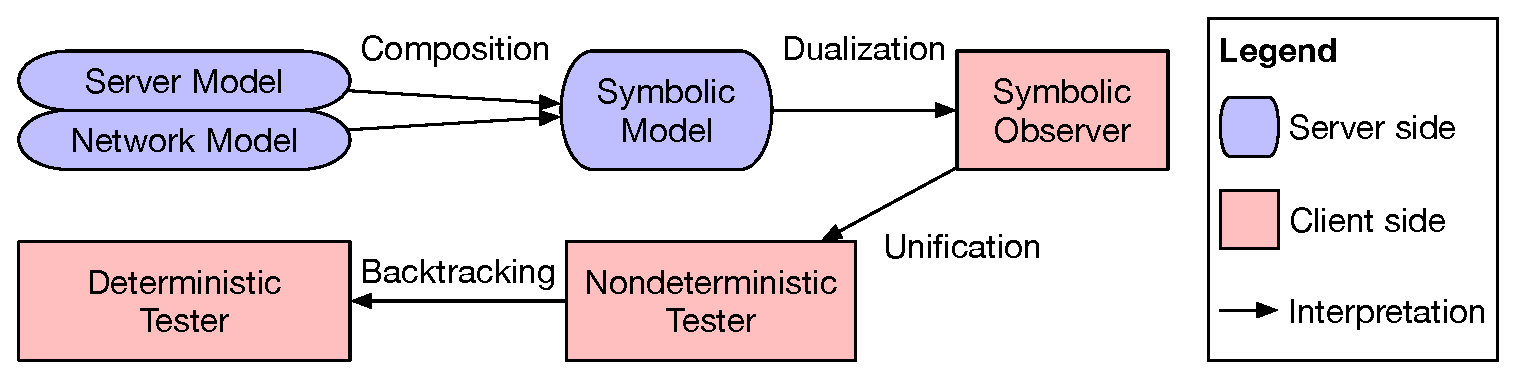
\includegraphics[width=\linewidth]{figures/framework}
  \caption{Deriving tester program from specification}
  \label{fig:framework}
\end{figure}

\section{Theories Developed for Interactive Testing}
\label{sec:previous-theories}
During the testing practice in \autoref{sec:practices}, the tester's quality was
evaluated by mutation testing, {\it i.e.} running the tester against buggy
implementations to see if it rejects.  To formally prove that the tester is
good, I develop a theory for reasoning on testers' good properties.

{\em Interactive testing} is a process that reveals the SUT's interactions and
determines whether it satisfies the specification.  There are two kinds of
interactions: (1) {\em inputs} that the tester can specify, and (2) {\em
  outputs} that are observed from the SUT.  In particular, when testing
networked systems, the input is a message sent by the tester, and the output is
a message received from the SUT.

When viewing the SUT as a function from inputs to outputs, we can test the
system by (1) providing an input, (2) get the output, and (3) validating the
input-output pair.  This process is called {\em synchronous testing}.

However, the nature of networked systems is that multiple messages might arrive
at the system simultaneously, and a high-throughput system should handle the
messages concurrently.  To check the system's validity upon concurrent inputs,
the tester should send multiple messages, rather than executing ``one client at
a time''.  This non-blocking process is called {\em asynchronous testing}.

My goal is to formalise the techniques in \textcite{issta21} into a generic
theory for asynchronous testing.

A tester consists of two parts: (i) a test harness that interacts with the SUT
and observes the interactions, and (ii) a validator that determines whether the
observations satisfy the specification.

The test harness needs to produce counterexamples effectively, and provide good
coverage of test cases.  The goal is to locate unknown bugs within a fixed
budget, which is more practical than theoretical, and will be discussed in
\autoref{sec:harness}.  The test theory in this dissertation focuses on
guaranteeing the soundness and completeness of the validator logic.

\subsection{Synchronous Testing Language}
Before facing the complexity in asynchronous testing, I start by formalising
synchronous testing theory, which describes how to build a sound and exhaustive
tester, and will expand the theory to asynchronous testing as described in
\autoref{sec:future-theories}.

\paragraph{Server specifications and validator implementations}
Synchronous testing can be viewed as a {\em server} interacting with a single
client, producing a {\em trace} of queries and responses, and a validator
determing whether the trace is acceptable or not.

\begin{definition}[Server model]
Let $Q$ be the query type, $A$ be the response type, $S$ be some server state,
then a deterministic server starts from an initial state, takes a query,
computes the response based on its current state, computes the next server
state, and loops over:
\[ \ottkw{DeterministicServer}\triangleq\sigT{S}{(Q \times S \to A \times S) \times S} \]

This definition is pronounced ``A deterministic server has some type $S$ that
represents its internal state.  It is specified by a step function of type
$Q\times S\to A\times S$, and an initial state of type $S$.''

In general, servers have {\em internal nondeterminism} that allows the responses
and transitions to depend on internal choices that are invisible to the testers,
{\it e.g.} timestamps and hash algorithms.  Let $C$ be the space of internal
choices, then a nondeterministic server is specified as:
\begin{align*}
  &\Server\triangleq\sigT{S}{(Q \times C \times S \to A \times S) \times S} \\
  &\stepServer:Q\times C \times \Server \to A\times \Server \\
  &\stepServer(q,c,\existT{S}{\sigma}{(\sstep, state)})\triangleq\\
  &\qquad\letin{(a,state')}{\sstep(q,c,state)} \\
  &\qquad(a, \existT{S}{\sigma}{(\sstep, state')})
\end{align*}
\end{definition}

Here $\existT{S}{\sigma}{(\sstep, state)}$ specifies a server whose internal
state type is $\sigma$, and has step function $(\sstep:Q\times C \times \sigma
\to A \times \sigma)$ and initial state $(state: \sigma)$.

\begin{definition}[Validator]
Let $V$ be some validator state, then a validator starts from an initial state,
takes a query and its corresponding response, determines whether these
interactions are valid, and computes the next validator state upon valid:
\begin{align*}
  &\Validator\triangleq\sigT{V}{(Q \times A \times V \to \option V) \times V} \\
  &\stepValidator:Q\times A \times \Validator \to \option \Validator \\
  &\stepValidator(q,a,\existT{V}{\beta}{(\vstep, state)})\\
  &\qquad\triangleq\begin{cases}
  \Some{(\existT{V}{\beta}{(\vstep,state')})} & \vstep(q,a,state)=\Some{state'} \\
  \None & \vstep(q,a,state)=\None
  \end{cases}
\end{align*}
\end{definition}

\paragraph{Deriving validator from server definition}
While it is possible to write server specifications and validators manually,
\textcite{issta21} have shown that internal nonderminism makes the
validator difficult to implement and reason about, and demonstrated how to
automatically derive a validator from a server specification.  That paper has
evaluated the derived validator's effectiveness by finding bugs in real world
programs, but did not provide a mathematical proof.  To construct a generic
derivation process, I start with a simplified derivation model for synchronous
tests.

\begin{definition}[Server and validator of a program]
  A program $p\in\Prog$ is a representation that can be ``instantiated'' into a
  server model:
  \[ \serverOf:\Prog\to\Server \]
  A program can also be ``interpreted'' into a validator:
  \[ \validatorOf:\Prog\to\Validator \]
\end{definition}

\paragraph{Soundness and completeness}
A tester is {\em sound} if any valid implementation passes it {\it i.e.} no
false rejection.  A tester is {\em exhaustive} if any invalid implementation
fails it (given sufficient time) {\it i.e.} no false acceptance.
\footnote{Concepts like ``sound'', ``complete'', ``false positive'', and ``false
  negative'' have opposite meanings in different contexts.  To avoid further
  confusion, I'll use ``reject'' and ``accept'' in place of ``positive'' and
  ``negative''.  The soundness and completeness definitions here is applied from
  \textcite{Tretmans}.}
  
A sound tester requires a sound validator, and a faithful test harness
that correctly interprets its observed behavior into the validator's input; An
exhaustive tester requires a {\em complete} validator, a faithful test harness,
plus an exhaustive test input generator that reveals all possible behavior of
the SUT.  Here I focus on the soundness and completeness of the validator.

\begin{definition}[Trace validity]
  A trace is valid if there exists an execution of the server model that {\em
    yields} it.  Let the trace be a list of query-response pairs $(\List
  (Q\times A))$, then:
  \begin{enumerate}
  \item Any server can step to itself, yielding an empty trace:
    \[\forall s\in\Server, \yields{s}{\nil}{s}\]
  \item A server yields a non-empty trace if it can yield the head of the trace
    and step into a server that yields the tail of the trace:
    \begin{align*}
      &\forall s,s_2\in\Server,\forall l\in\List(Q\times A),\forall q\in Q,\forall a\in A,\\
      &(\exists s_1\in\Server,\exists c\in C\mid\yields{s}{l}{s_1}\wedge
      \stepServer(q,c,s_1)=(a,s_2)) \\
      &\implies \yields{s}{l+(q,a)}{s_2}
    \end{align*}
  \end{enumerate}
\end{definition}

\begin{definition}[Trace acceptance]
  A trace is {\em accepted} by a validator if the validator consumes the entire
  trace and steps into a nonempty state:
  \begin{enumerate}
  \item Any validator accepts an empty trace and steps to itself:
    \[ \forall v\in\Validator,\accepts{v}{\nil}{v} \]
  \item A validator accepts a non-empty trace if it can consume the head of the
    trace and step into a validator that accepts the end of the trace:
    \begin{align*}
      &\forall v,v_2\in\Validator,\forall
      l\in\List(Q\times A),\forall q\in Q, \forall a\in A, \\
      & (\exists v_1\in\Validator\mid\accepts{v}{l}{v_1}\wedge
      \stepValidator(q,a,v_1)=\Some{v_2}) \\ &\implies
      \accepts{v}{l+(q,a)}{v_2}
    \end{align*}
  \end{enumerate}
\end{definition}

\begin{definition}[Soundness]
  A validator is {\em sound} per server specification if it accepts all valid
  traces of the specification:
  \[ \issound{v}{s}\triangleq\forall l\in\List(Q\times A),(\exists s'\in\Server\mid\yields{s}{l}{s'})\implies\exists v'\in\Validator\mid\accepts{v}{l}{v'} \]
\end{definition}

\begin{definition}[Completeness]
  A validator is {\em complete} per server specification if it only accepts valid
  traces of the specification:
  \[ \iscomplete{v}{s}\triangleq\forall l\in \List(Q\times A),(\exists{v'}\in\Validator\mid\accepts{v}{l}{v'})\implies\exists{s'}\in\Server\mid\yields{s}{l}{s'} \]
\end{definition}

\subsection{Reasoning on Synchronous Testers}
\label{sec:sync-reasoning}

Given a server $\existT{S}{S}{(\sstep, s_0)}$ and a validator
$\existT{V}{V}{(\vstep,v_0)}$, to prove its soundness and completeness, we need to
show properties over the step functions and the initial states.

The validator's soundness says: For any trace producable by the server
specification, that trace can be accepted by the validator.  The completeness
says: For any trace accepted by the validator, there exists an execution of the
server specification that yields this trace.

Since the server and validator are both loops, I introduce an invariant
$\{\Reflects{v}{s}\mid v\in V,s\in S\}$, which is preserved by the loops' step
functions.

\paragraph{Proving soundness}
The soundness proof is by forward induction of the server execution path, and
construct the corresponding validation path based on the following assumptions:

\begin{enumerate}
\item The initial server state reflects the initial validator state:
  \[ \Reflects{v_0}{s_0} \]
\item Any server step whose pre-execution state reflects some pre-validation
  state can be consumed by the validator into a post-validation state that
  reflects the post-execution state:
  \begin{align*}
    &\forall q\in Q,\forall c\in C,\forall a\in A,\forall s,s'\in S,\forall v\in V,\\
    &\sstep(q,c,s)=(a,s')\wedge\Reflects{v}{s}\\
    &\implies\exists v'\in V,\vstep(q,a,v)=\Some{v'}\wedge\Reflects{v'}{s'}
  \end{align*}
  \begin{center}
    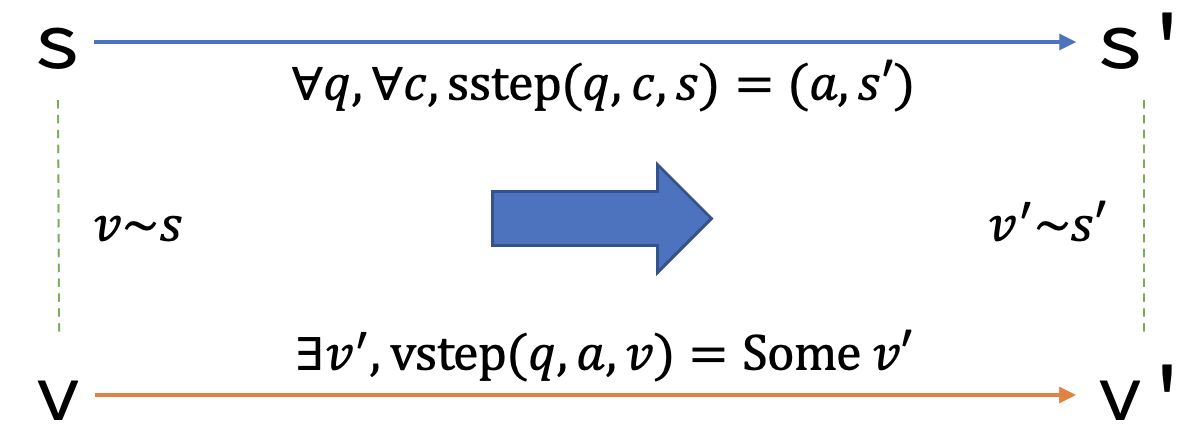
\includegraphics[width=.5\textwidth]{figures/soundness-preservation}
  \end{center}
\end{enumerate}

\paragraph{Proving completeness}
The completeness proof is by backward induction of the validation path, and
construct the corresponding server execution path based on the following
assumptions:

\begin{enumerate}
\item Any accepting validator step has some server state that reflects the
  post-validation state:
  \begin{align*}
    \forall q\in Q,\forall a\in A,\forall v, v'\in V,\;&\vstep(q,a,v)=\Some{v'}\\
    &\implies\exists s'\in S,\Reflects{v'}{s'} 
  \end{align*}
\item Any accepting validator step whose post-validation state reflects some
  post-execution server state has a corresponding server step from a
  pre-execution state that reflects the pre-validation state:
  \begin{align*}
    &\forall q\in Q,\forall a\in A,\forall v,v'\in V,\forall s'\in S,\\
    &\vstep(q,a,v)=\Some{v'}\wedge\Reflects{v'}{s'}\\
    &\implies\exists c\in C,\exists s\in S,\sstep(q,c,s)=(a,s')\wedge\Reflects{v}{s}
  \end{align*}
  \begin{center}
    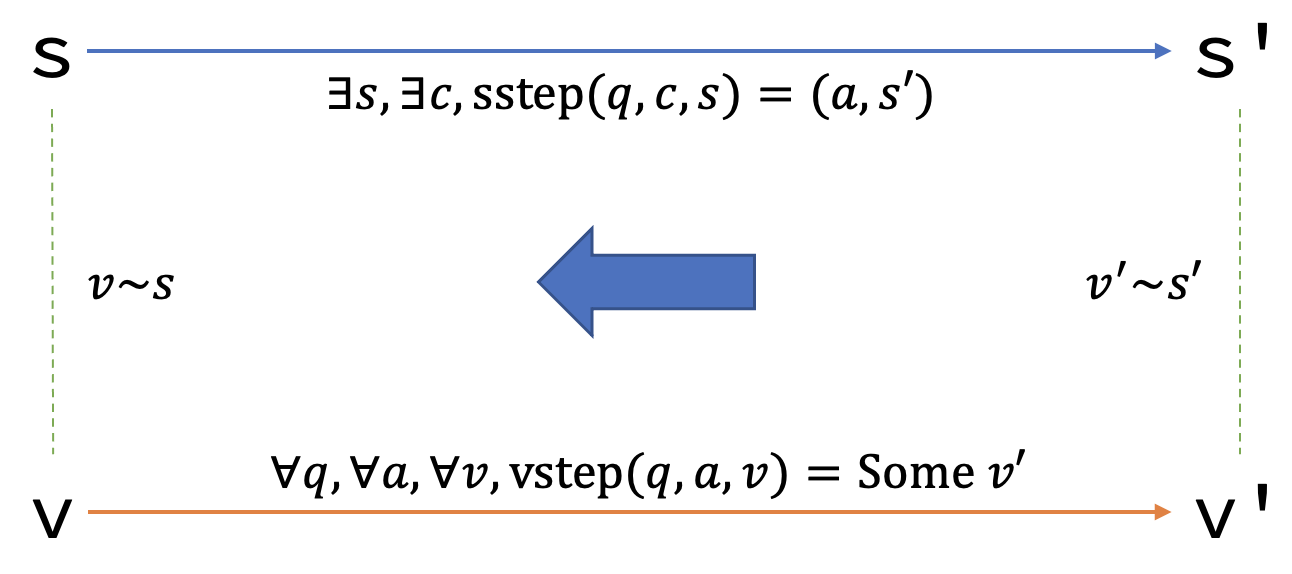
\includegraphics[width=.5\textwidth]{figures/completeness-preservation}
  \end{center}

\item The initial validator state only reflects the initial server state:
  \[\{s\mid\Reflects{v_0}{s}\}=\{s_0\}\]
\end{enumerate}

\subsection{Case Study: Single Instruction Server}
\label{sec:opserver}

In this experiment, I target a simple server language where the program is a
single instruction.  I'll show how to instantiate the program into a server
model, and how derive the program into a validator that is sound and complete.
That is, defining $\serverOf$ and $\validatorOf$ functions for $\Prog$ such
that:

\begin{align*}
  \forall p:\Prog,\;&\letin{s}{\serverOf(p)}\\
  &\letin{v}{\validatorOf(p)}\\
  &\issound{v}{s}\wedge\iscomplete{v}{s}
\end{align*}

\paragraph{Server language}
The server stores a key-value mapping $K\to\Nat$.  The server program is a
three-address instruction that performs an arithmetic operation:
\[\Prog \triangleq \{!dst\gets !src_1\;op\;!src_2\mid op\in\{+,-,\times,\div\};
dst,src_1,src_2\in K\}\]

A program in this language is instantiated into a server step as follows: Upon
receiving a query $q\in Q$, the server writes a choice $c\in C$ to key 1, and
writes the query to key 0.  The server then runs the instruction, and sends back
the value stored in key 0:

\begin{align*}
  \rlap{$Q\triangleq\Nat\qquad C\triangleq\Nat\qquad A\triangleq\Nat$}\\
  \rlap{$\serverOf(p)\triangleq\existT{S}{(K\to\Nat)}{(\sstep(p), (\_\mapsto0))}$}\\
  \rlap{where}\\
  \rlap{$\sstep(!dst\gets !src_1\;op\;!src_2)(q,c,s_0)\triangleq$}\\
  &\qquad\letin{s_1}{s_0 [k_1\mapsto c]}\\
  &\qquad\letin{s_2}{s_1 [k_0\mapsto q]}\\
  &\qquad\letin{s_3}{s_2 [dst\mapsto s_2(src_1)\;op\;s_2(src_2)]}\\
  &\qquad(s_3(k_0), s_3)
\end{align*}

To check a trace against this server model, the validator introduces symbolic
variables $x\in X$ to represent the values stored in each key.  The validator
also maintains a set of constraints that reflect the server's computations:

\begin{align*}
  \rlap{$E\triangleq\; \Nat \cup \{!x\mid x\in X\} \cup \{!x_1\;op\;!x_2\mid
    op\in\{+,-,\times,\div\}; x_1,x_2\in X\}$}\\
  \rlap{$\Constraint\triangleq\{e_1=e_2\mid e_1,e_2\in E\}$}\\
  \rlap{$\beta\triangleq(K\to X)\times\List\Constraint$}\\
  \rlap{$\validatorOf(p)\triangleq\existT{V}{\beta}{(\vstep(p), ((\_\mapsto x_0),(0=\;!x_0)))}$}\\
  \rlap{where}\\
  \rlap{$\vstep(p)(q,a,v_0)\triangleq\;$}\\
  &\qquad\letin{v_1&}{\;&\Havoc(k_1,v_0)&}\\
  &\qquad\letin{v_2&}{\;&\Write(k_0,q,v_1)&}\\
  &\qquad\letin{(vs_3,cs_3)&}{\;&\Exec(p,v_2)&}\\
  &\qquad\letin{cs_4&}{\;&cs_3+(!vs_3(k_0)=a)&}\\
  \rlap{$\qquad\If \solvable(cs_4)\;\Then \Some{(vs_3,cs_4)}\;\Else \None$}\\
  \rlap{$\Write(k,q,(vs,cs))\triangleq$}\\
  \rlap{$\qquad\letin{x}{\fresh(vs,cs)}$}\\
  \rlap{$\qquad(vs[k\mapsto x],cs+(q=\;!x))$}\\
  \rlap{$\Havoc(k,(vs,cs))\triangleq$}\\
  \rlap{$\qquad\letin{x}{\fresh(vs,cs)}$}\\
  \rlap{$\qquad(vs[k\mapsto x],cs)$}\\
  \rlap{$\Exec((!dst\gets\;!src_1\;op\;!src_2),(vs,cs))\triangleq$}\\
  \rlap{$\qquad\letin{x}{\;\fresh(vs,cs)}$}\\
  \rlap{$\qquad(vs[dst\mapsto x],cs+(!vs(src_1)\;op\;!vs(src_2)=\;!x))$}\\
  \rlap{$\fresh:\beta\to X$}\\
  \rlap{$\solvable:\List\Constraint\to\bool$}
\end{align*}

When the $\sstep$ function modifies the server state, the $\vstep$ function
updates the validator's view of the server correspondingly: When the server
stores a query to key 0, the $\Write$ function maps key 0 to a $\fresh$
variable, and adds a constraint that the variable's value is equal to the query.
When the server stores an internal choice to key 1, the $\Havoc$ function maps
key 1 to a fresh variable with no constraints, because its exact value is
invisible to the validator.  When the server runs a three-address instruction,
the $\Exec$ function maps the destination to a fresh variable, and adds a
constraint that the variable's value should reflect the three-address
computation.

After updating its symbolic view of the server, the validator expects the
observed response to be explainable by its symbolic view.  Such expectation is
checked by a constraint solver, that determines whether the constraints can be
satisfied by some assignment of the variables:

\begin{align*}
  \Assignment\triangleq\;&X\to\Nat\\
  \Evaluate\quad:\;&\Assignment\times E\to\Nat\\
  \Satisfy(asgn,cs)\triangleq\;&\forall (e_1=e_2)\in cs,\\
  &\Evaluate(asgn,e_1)=\Evaluate(asgn,e_2)\\
  \forall cs\in\List{\Constraint},\;&\solvable(cs)\\
  &\iff\exists\; asgn\in\Assignment,\Satisfy(asgn,cs)
\end{align*}

To prove the validator's completeness, the reflection relation is defined as:

\begin{align*}
  (\Reflects{(vs,cs)}{s})\triangleq\exists\;asgn,\;&\Satisfy(asgn,cs)\\
  &\wedge \forall k\in K,asgn(vs(k))=s(k)
\end{align*}

This reflection definition is sufficient for proving the validator's
completeness, as it satisfies all the assumptions in \autoref{sec:sync-reasoning}:

\begin{enumerate}
\item Any accepting validator step has solved the post-validation constraints
  $cs'$, which implies an assignment $asgn$ that satisfies $cs'$.  Let $vs'$ be
  the post-validation key-variable mapping, then $s'=asgn\circ vs'$ reflects the
  post-validation state $(vs',cs')$ by definition.

\item The $\vstep$ function monotonically increases the list of constraints, and
  thus monotonically narrows the space of satisfying assignments.  Let $s'$ be
  the post-execution server state that reflects the post-validation state
  $(vs',cs')$, then $asgn$ is guaranteed to satisfy the pre-validation
  constraints $cs$.  Therefore, by analysing the execution of
  $\vstep(q,a,(vs,cs))$, we can construct the pre-execution server state
  $s=asgn\circ vs$ and the server's internal choice $c=asgn(\fresh(vs,cs))$ that
  satisfy $\sstep(q,c,s)=(a,s')$ and $\Reflects{(vs,cs)}{s}$.

\item From the definition of the server and validator's initial state, we can
  show that the initial server state is the only state that reflects the initial
  validator state.
\end{enumerate}

The soundness proof is pending, but I've proven the soundness of validators for
a simpler server language.

\section{Research Plan}
\label{sec:research-plan}

\subsection{Theories of Interactive Testing}
\label{sec:future-theories}

\paragraph{Synchronous Testing in General}
The server language shown in \autoref{sec:opserver} consists of a single
instruction.  I plan to extend that language with sequential combinators and
If-branches, for modelling more realistic server programs.  For example:

\begin{lstlisting}[style=customcoq]
  Inductive Prog: Type :=
    Singleton (i: Instruction)
  | Sequence  (p1 p2: Prog)
  | Branch    (condition: Expression) (thenP elseP: Prog).
\end{lstlisting}

This language covers a subset of C programs, excluding loops with indefinite
iterations (which is not common in server programs' control flow).  It can also
model various implementation choices, using \ilc{Branch c p1 p2} where the
\ilc{c}ondition is an unbound variable.

\paragraph{Asynchronous Testing}
The server model in \autoref{sec:sync-reasoning} has separated the computations
from the interactions.  To model asynchronous interactions of the server, I plan
to merge the send/receive interactions into the server language, between the
lines of computations.  For example:

\begin{lstlisting}[style=customcoq]
  Inductive Prog  : Type :=
    Recv (handler : Message -> Prog)
  | Send (response: Message)
  | Singleton ...
  | Sequence ...
  | Branch ...
  | ...
\end{lstlisting}

\subsection{Test Input Generation and Shrinking Techniques}
\label{sec:harness}
To make a sound and exhaustive tester useful in software engineering practices,
we need to (1) generate test inputs that can reveal potential bugs quickly, and
(2) report minimal counterexamples to debuggers, rather than thousand-line logs.

One challenge for random testing is that, to find failing examples efficiently,
it is important to generate fairly large test cases.  But then, after a failing
test case has been found, it is important to \textit{minimize} the test input to
eliminate the parts that are not relevant to provoking the failure.  Tools like
QuickCheck therefore provide automatic methods for minimizing, or {\em
  shrinking}, failing tests, by incrementally generating smaller variants until
they reach a local minimum---a counterexample that cannot be reduced any
further.

Traditional shrinking doesn't work well for impure programs, which might mutate
state or interact with their environments, because an interesting test input in
one execution might become trivial or irrelevant in another run.  In particular,
when testing an interactive program, interesting test inputs might depend on
existing observations of the program's behavior.

To generate and shrink inputs that are interesting among different executions,
\textcite{Hughes2007} introduced a method that relates inputs to runtime
observations.  In this framework, the tester interacts with the system under
test (SUT) via function calls, and maintains a runtime state that is updated
after each call returns.  Test inputs are represented in an abstract language
that depends on the runtime state {\it e.g.} ``call function \ilc{foo(x)}, where
\ilc{x} is the return value of the 10th function call''.  Such abstract
representation is instantiated into a concrete input during runtime, by
remembering the 10th call's return value \ilc{a} to build the actual function
call \ilc{foo(a)}.

This methodology has achieved good results in testing state
machines~\cite{Hughes2016}, but the specification language requires the
interactions to be synchronous {\it i.e.} to return immediately upon call.
However, when testing networked systems, requests and responses might be delayed
or reordered \textit{en route}.  Such a scenario requires a different
specification language that allows asynchronous
interactions~\cite{issta21}, introducing new challenges in minimizing
test inputs, {\it e.g.} when a dependent response has not arrived.

I'll propose a generic method for generating and minimizing asynchronous test
interactions, by combining the idea of abstract input representation
from~\textcite{Hughes2007} with the asynchronous specification language
of~\textcite{issta21}.  The tester records a {\em trace} of network
packets sent and received, and uses the trace to instantiate abstract inputs
into concrete requests to send.  The key inovation is an intermediate
representation (IR) between structured application messages and bytes.  The IR
allows the generated abstract input to refer to specific fields in the trace,
and can handle situations where the referred field is absent (caused by internal
or network nondeterminism).

A preliminary design is shown in \autoref{sec:appendix-ir}.

\section{Evaluation Criteria}
\label{sec:criteria}

As mentioned in \autoref{sec:intro}, this thesis is to propose language designs
for (i) validation logic and (ii) test case generation, and provide an
asynchronous testing methodology with (i) theoretical guarantee of soundness and
completeness, and (ii) practicality in testing real-world applications.

\subsection{Practices: Testing More Complex Network Applications}
To demonstrate the specification language's expressiveness and the derived
tester's effectiveness, I'll apply my test framework to a web application on top
of \http.

\paragraph{Protocol specification}
I'll develop a simple exchange where users can trade assets by placing orders.
The application specification for the exchange's functionality will be composed
with the underlying \http specification, to show that specifications written in
my language are reusable and can be developed modularly.

\paragraph{Test case generation}
The exchange server will communicate with clients using JSON, a common message
format for web applications.  My tester will generate requests using flexible
heuristics, that can refer to fields in JSON's data strucutre which can be
arbitrarily deep.

\paragraph{Research questions}
\begin{enumerate}
\item For testing nontrivial protocols, is the specification easy to write and
  easy to understand?
\item Can the derived tester effectively produce minimal counterexamples and
  help debugging server implementations?
\end{enumerate}

\subsection{Theories: Verified Testing Framework}
To show the methodology of formally reasoning of derived testers, I'll extend
the server language $\Prog$ as proposed in \autoref{sec:future-theories}, such
that a nontrivial application can be written in this language.  I'll then
implement the $(\validatorOf:\Prog\to\Validator)$ algorithm, and prove its
soundness and completeness.

The experiments with \http are conducted with ITrees, whereas the $\Prog$ is a
tree of imperative instructions.  While bridging the language gap in between is
beyond the scope of this thesis, I'd expect the reasoning methods here can
inspire test developers of other languages.

\paragraph{Research questions}
\begin{enumerate}
\item As the $\Prog$ language extends, how to adjust the verification framework
  to prove validators' soundness and completeness?
\item Can the proof technique for $\Prog$-based validators be applied to other
  specification languages, {\it e.g.} interaction trees?
\end{enumerate}

\printbibliography
\pagebreak

\appendix
\section{Language Design for Test Generation}
\label{sec:appendix-ir}
\subsection{Overview}
\begin{figure}
  \centering
  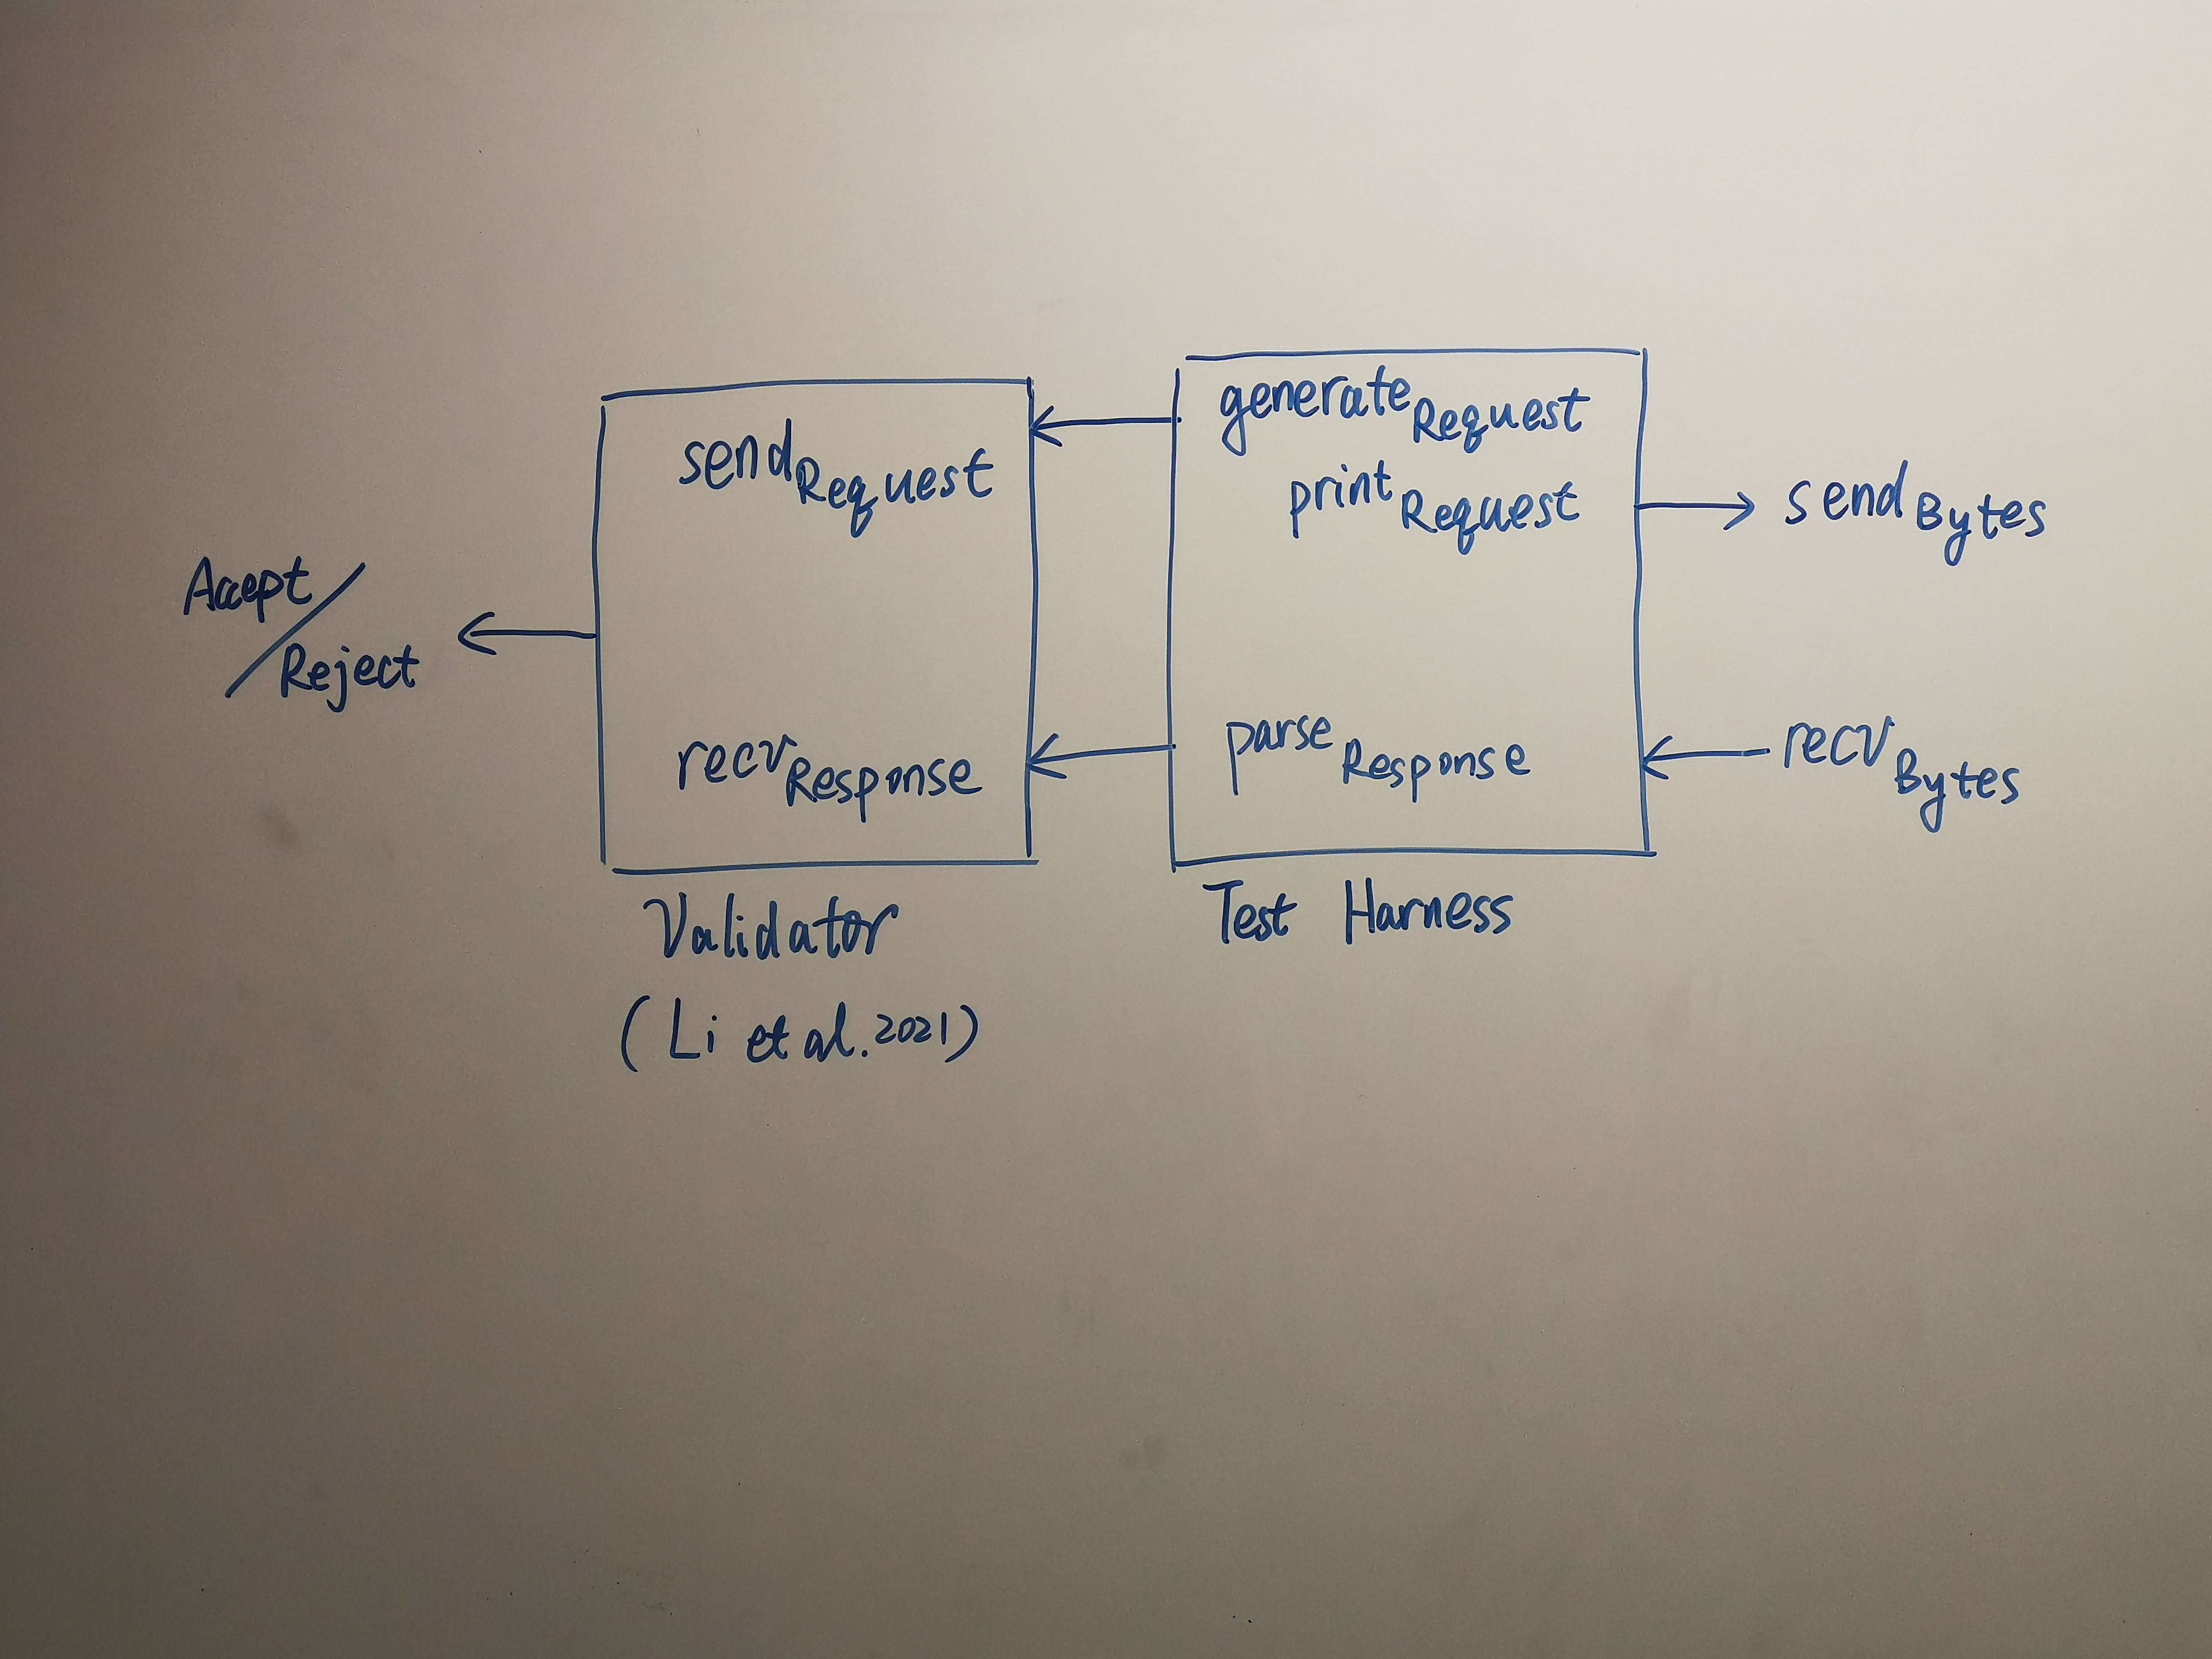
\includegraphics[width=.9\textwidth]{figures/overview}
  \caption{Test framework overview}
  \label{fig:overview}
\end{figure}

As shown in \autoref{fig:overview}, the test framework consists of a {\em
  validator} that determines whether the SUT's behavior satisfies the
specification, and a {\em test harness} that provides test inputs for the
validator.

A {\em validator} is a client-side model program that observes messages sent and
received and decides whether these interactions are conformant to the
specification.  For example, a simple validator for echo server is written as:
\begin{lstlisting}[style=customcoq]
  let validateEcho =
    request := sendRequest();
    response := recvResponse();
    if response <> request
    then reject
    else validate
\end{lstlisting}
Notice that the \ilc{sendRequest} event does not take the request to be sent as
argument, but in stead returns the request actually sent.  The validator only
describes the logic that checks messages sent and received, while the test
harness computes what requests to send.

The {\em test harness} takes a validator and turns it into an executable program
that performs network interactions.  It handles the validator's send and receive
events, and generates the requests to be sent.  A simple test harness for the
validator above is written as:
\begin{lstlisting}[style=customcoq]
  let execute(v) =
    match v with
    | x := sendRequest(); v'(x) =>
      request := arbitraryRequest();
      sendBytes(print(request));
      execute(v'(request))
    | x := recvRequest(); v'(x) =>
      responseBytes := recvBytes();
      execute(v'(parse(responseBytes)))
    | reject => reject
    end in
  execute(validateEcho)
  (* ... is equivalent to ... *)
  let executeValidateEcho =
    request := arbitraryRequest();
    sendBytes(print(request));
    responseBytes := recvBytes();
    if parse(responseBytes) <> request
    then reject
    else executeValidateEcho
\end{lstlisting}

The \ilc{arbitraryRequest} generator here produces requests randomly.  To
generate requests that depend on previously observed messages, my framework will
extend the test harness in \autoref{fig:overview} that records a trace of
messages.

\subsection{Architecture}
\begin{figure}
  \centering
  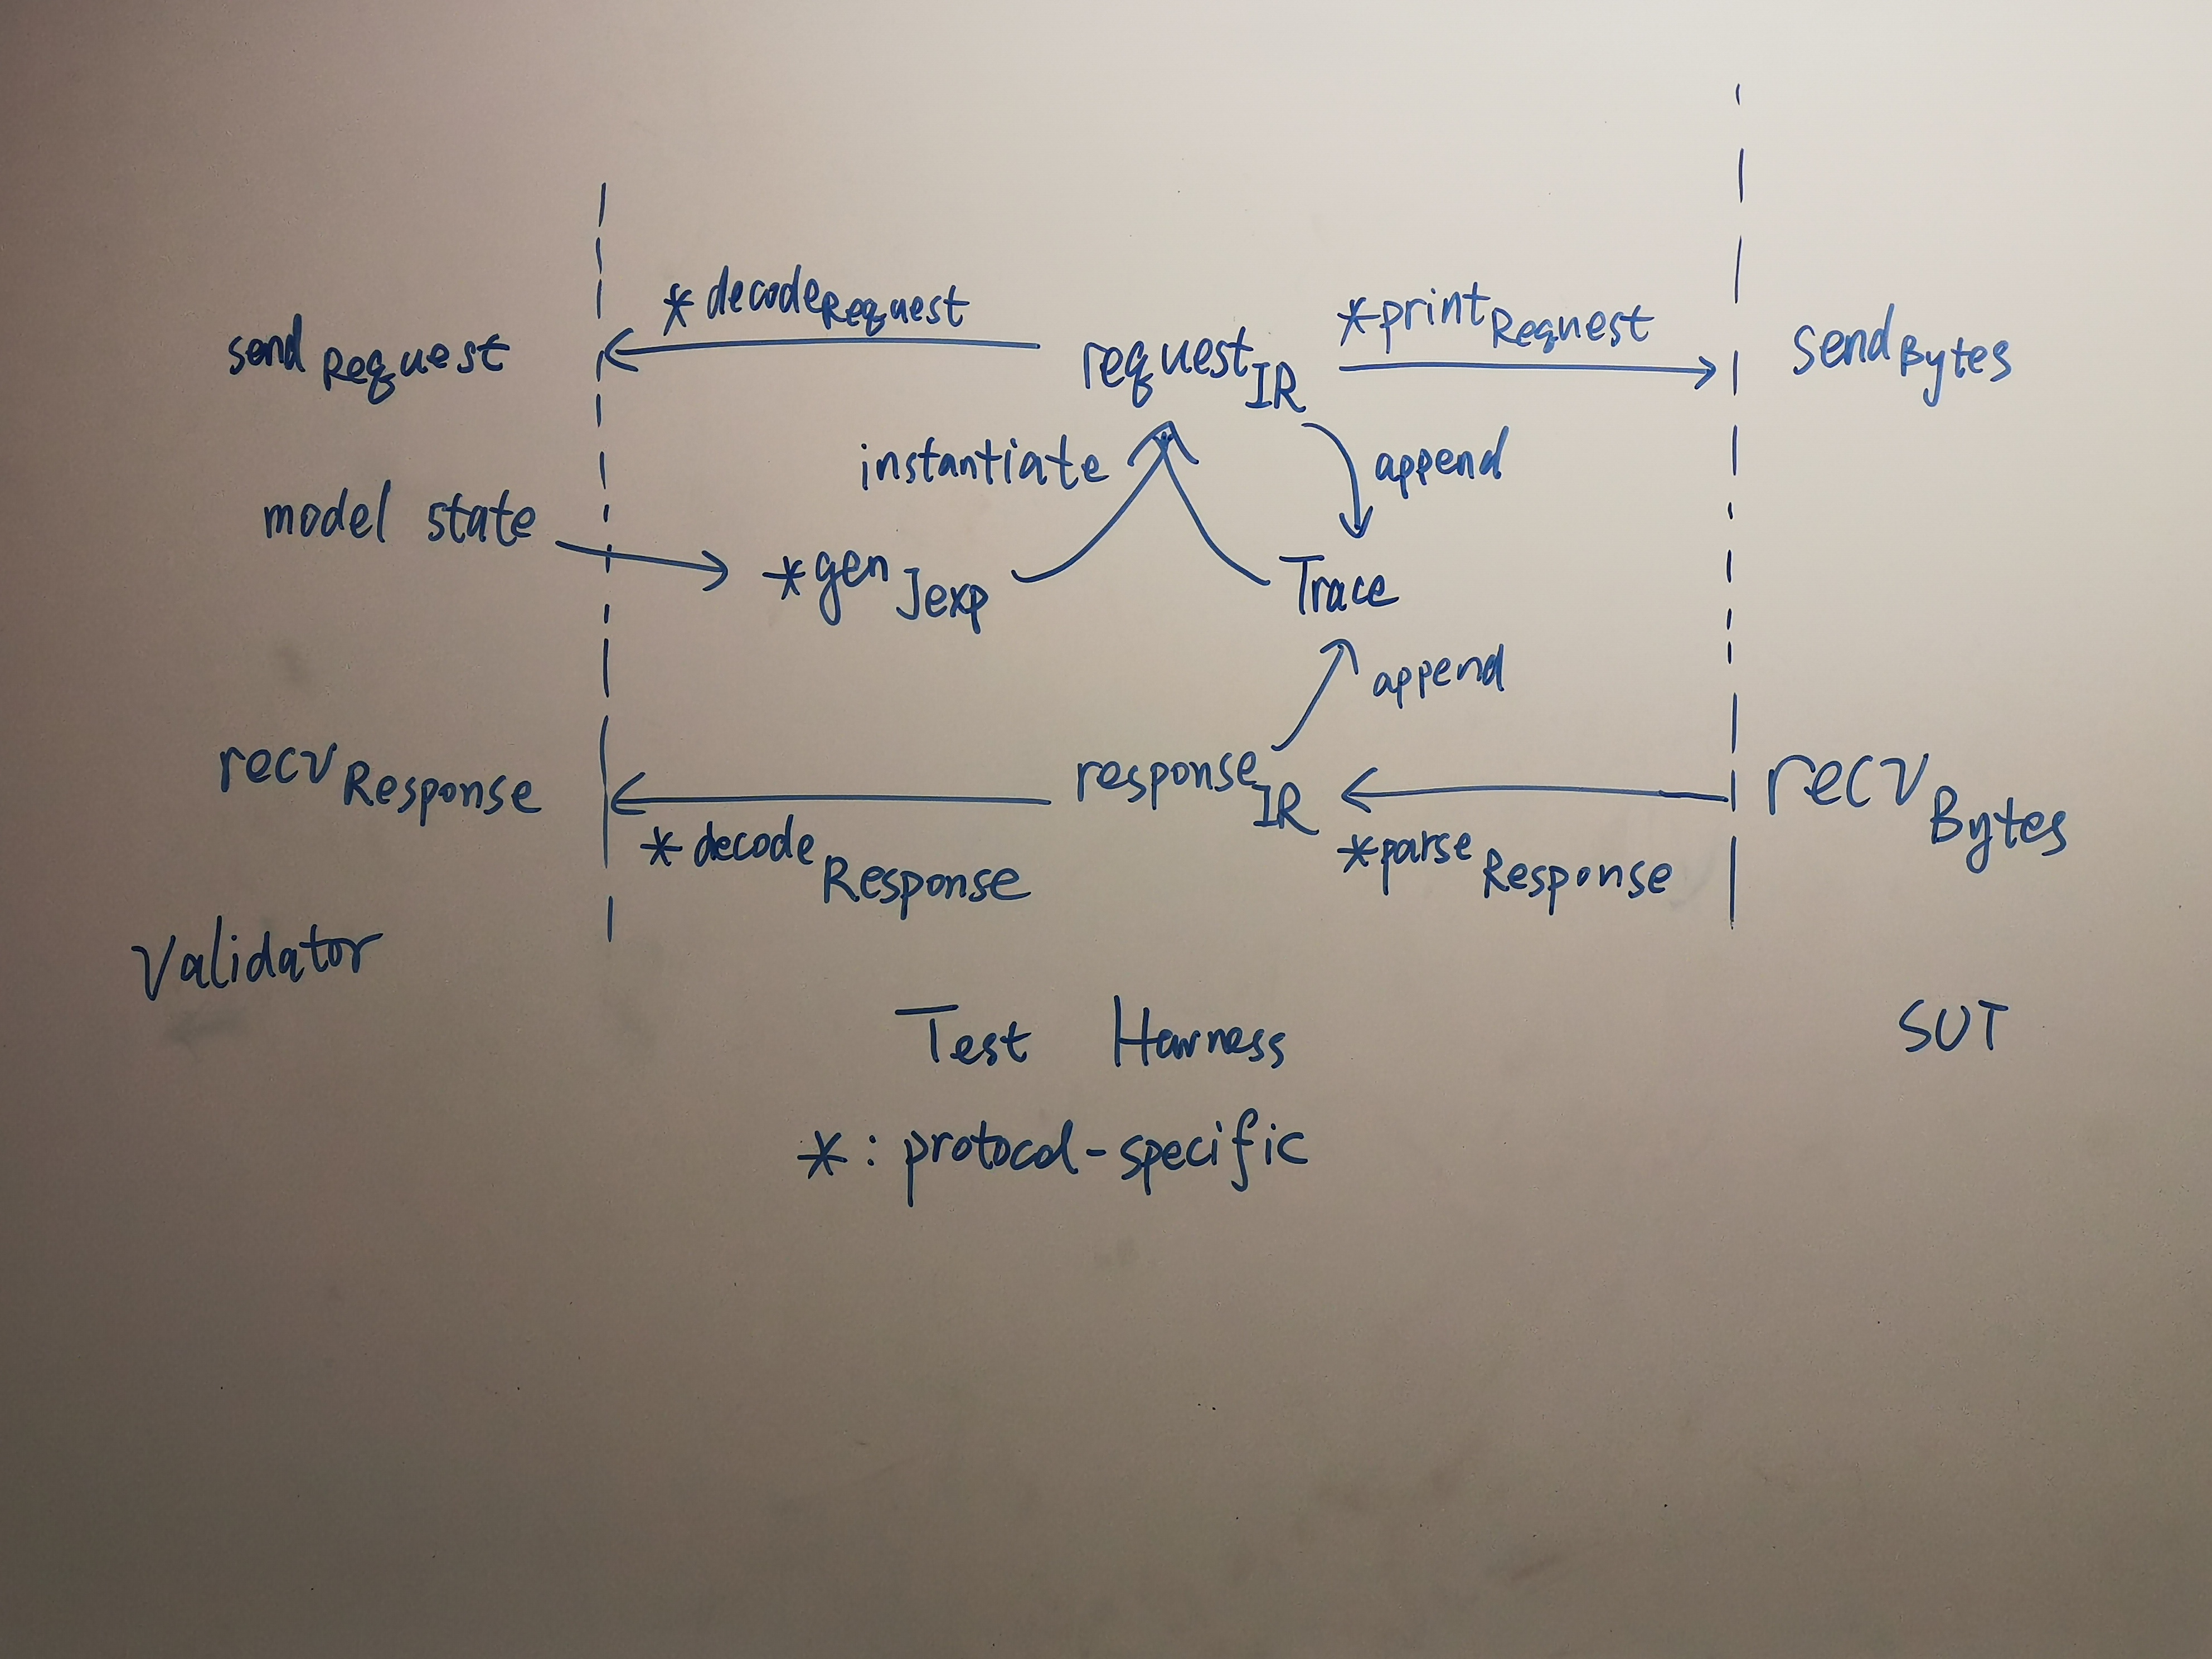
\includegraphics[width=.8\textwidth]{figures/harness}
  \caption{Test harness mechanism}
  \label{fig:harness}
\end{figure}

As shown in \autoref{fig:harness}, the test harness records a trace of requests
and responses, using an generic intermediate representation.  Requests are
generated as ``J-expressions'' that can be instantiated into a request IR based
on the trace.  For each protocol to test, the developers need to specify how to
generate J-expressions that represent requests.  Developers also need to define
how to interpret among the IR, bytes, and application messages.

\subsection{Intermediate representation language}
The purpose of introducing an IR in this framework is to enable a generic method
for generating requests that refer to specific fields in the trace.  For
example, when testing conditional HTTP requests, the generator wants to include
``a precondition that uses the ETag field of a previous response''; when testing
an online store, the generator wants to provide ``an order ID that the server
has mentioned before''.

I choose JSON as the intermediate representation.  Since JSON itself is widely
used in web applications, the IR should provide the flexibility for developers
to refer to any field in a JSON message, which might involve arbitrarily deep
path down the syntax tree.  \autoref{fig:ir} shows the intermediate
representation for two protocols.

\begin{figure}
  \begin{lstlisting}[style=customcoq]
    Example response1 : http_response :=
      Response (Status (Version 1 1) 200 (Some "OK"))
               [Field "ETag" "tag-foo";
                Field "Content-Length" "11"]
               (Some "content-bar").

    Example response2 : store_response :=
      Response__ListOrders [(233, (12, 100, 34, 500));
                            (996, (56, 400, 78, 20))].
  \end{lstlisting}
  \begin{minipage}[t]{.4\textwidth}
    \begin{lstlisting}[style=json]
      {
        "version": {
          "major": 1,
          "minor": 1
        },
        "code": 200,
        "reason": "OK",
        "fields": {
          "ETag": "tag-foo",
          "Content-Length": "11"
        },
        "body": "content-bar"
      }
    \end{lstlisting}
  \end{minipage}%
  \begin{minipage}[t]{.4\textwidth}
    \begin{lstlisting}[style=json]
      {
        "code": 200,
        "orders": [
          {
            "ID": 233,
            "BuyerID": 12,
            "BuyAmount": 100,
            "SellerID": 34,
            "SellAmount": 500
          },
          {
            "ID": 996,
            "BuyerID": 56,
            "BuyAmount": 400,
            "SellerID": 78,
            "SellAmount": 20
          }
        ]
      }
    \end{lstlisting}
  \end{minipage}
  \caption{Application message example for HTTP and online store protocols, and
    their corresponding intermediate representation}
  \label{fig:ir}
\end{figure}

To represent the correspondence between requests and responses, the trace labels
each message, and the request-response pair have the same label.
\autoref{fig:trace} shows a trace of messages sent and received by the tester
client.

\begin{figure}
  \begin{minipage}{.5\textwidth}
    \begin{lstlisting}[style=json]
      [
        {
          "label": 10,
          "message": {
            "method": "GET",
            "path": "index.html"
          }
        },
        {
          "label": 20,
          "message": {
            "method": "DELETE",
            "path": "index.html"
          }
        },
        {
          "label": 20,
          "message": {
            "code": 204,
            "reason": "No Content",
          }
        },
        {
          "label": 10,
          "message": {
            "code": 410,
            "reason": "Gone"
          }
        }
      ]
    \end{lstlisting}
  \end{minipage}%
  \begin{minipage}{.5\textwidth}
    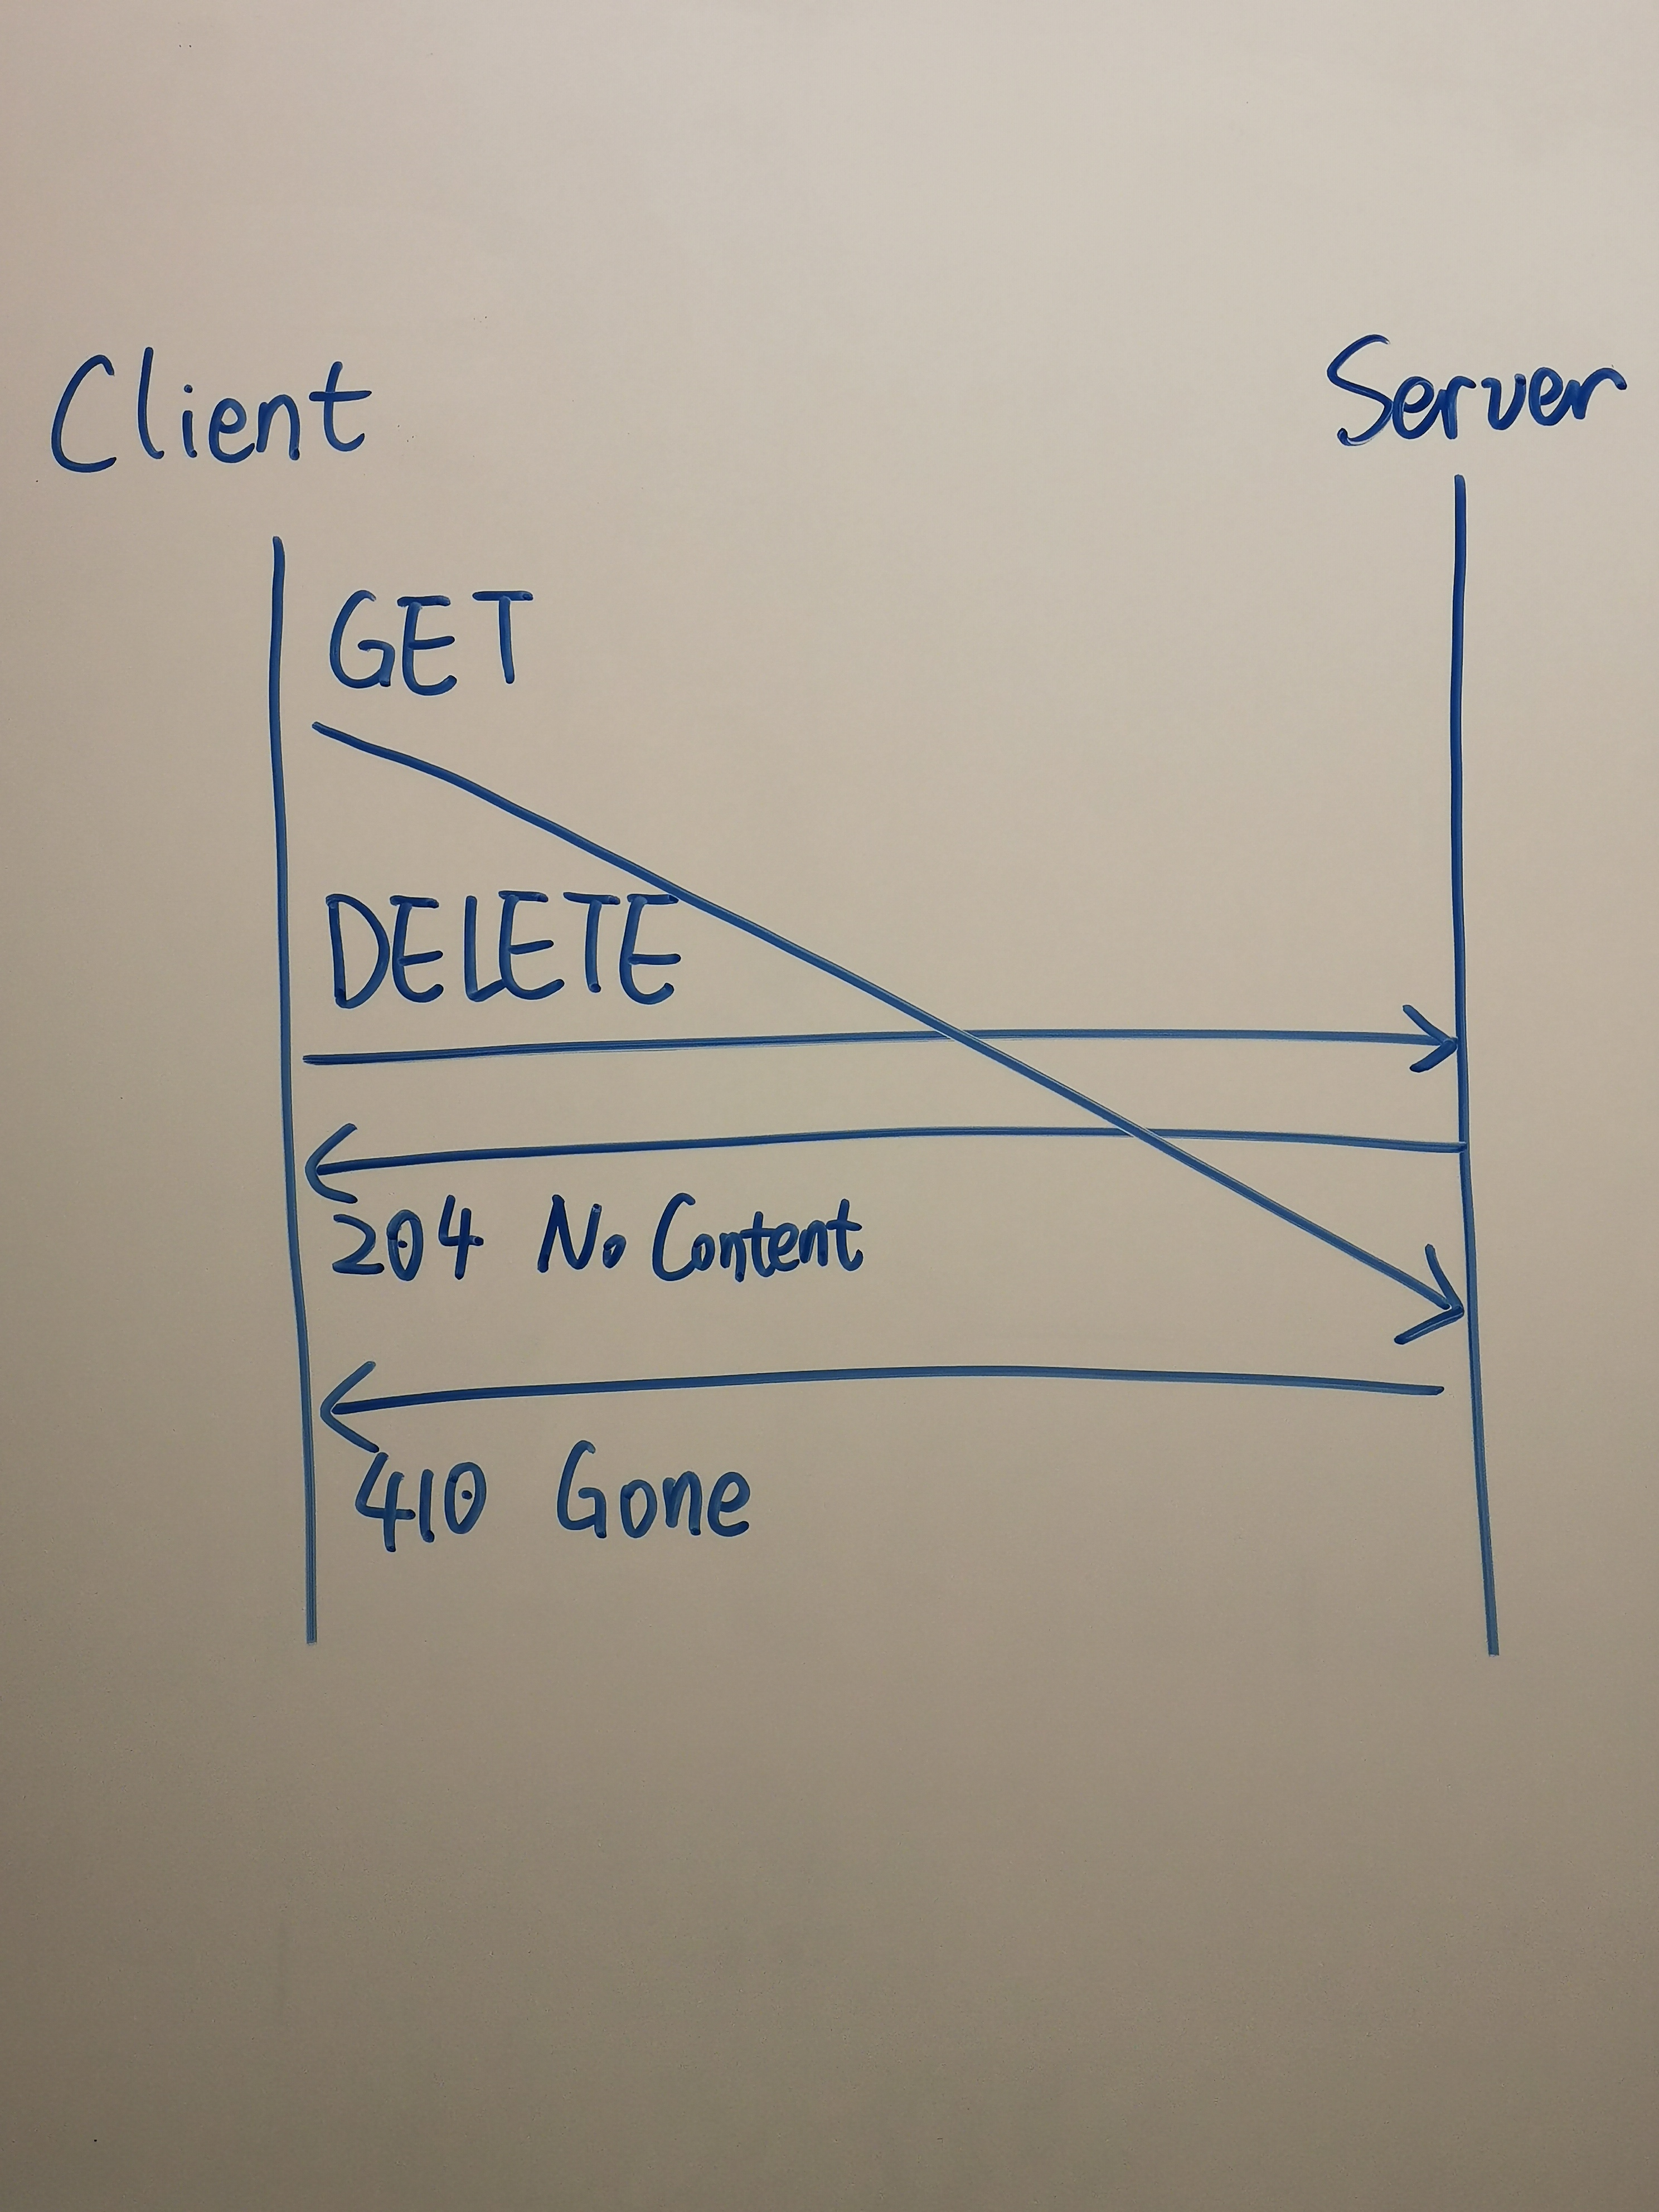
\includegraphics[width=\textwidth]{figures/trace}
  \end{minipage}
  \caption{Example client-side trace and its corresponding IR}
  \label{fig:trace}
\end{figure}

\begin{figure}
  \ottall
  \caption{Formal definition of J-expressions}
  \label{fig:jexp}
\end{figure}

Based on this unified structure of messages, I introduce a symbolic language for
representing requests, called ``J-expressions'', defined in \autoref{fig:jexp}.
The J-expression is similar to JSON, except that it allows a pointer notation
that refers to the trace.  For example, the following J-expression represents a
\ilc{takeOrder} request whose order ID is equal to the second order's ID in the
message labelled 30:
\begin{lstlisting}[style=json]
  {
    "method": "takeOrder",
    "user": 2,
    "order": ref 30 (this@"orders"#2@"ID") id
  }
\end{lstlisting}

Notice the \ilc{ref} in the final line: The first argument 30 is the message
label in the trace.  The following \ilj{this@"orders"#2@"ID"} is a path for the
generator to search in the IR, pronounced ``the `ID' field in the 2nd entry of
the array named `orders' ''.  The last argument is the transformer function that
maps the found field to the generated request, here \ilj{id} is the identical
function, meaning the found order ID is used in the result request verbatim.

Suppose a trace contains a message labelled 30, and its payload is the second
example in \autoref{fig:ir}, then the request generator can find the
corresponding order ID in the request {\it i.e.}  996, and construct the
following request IR based on the J-expression above:

\begin{lstlisting}[style=json]
  {
    "method": "takeOrder",
    "user": 2,
    "order": 996
  }
\end{lstlisting}

\subsection{Instantiating J-expression into request IR}
Suppose the test developer has generated some J-expression to represent request
to send, the tester harness needs to instantiate the J-expression into the
request IR.  In particular, \ilj{ref} expression referrs to a field in the
trace, so the test harness should locate its corresponding value.

When testing networked systems, response packets might be delayed by the
network.  As a result, when the tester wants to send a request that depends on a
response labelled $l$, it is possible that the response hasn't arrived yet.  In
this case, to avoid blocking the program, the test harness should find some
fallback options to instantiate the J-expression.  A useful solution is to
ignore the label and find if any message in the trace has a field of the given
J-path.

Even if the labelled response has arrived, considering internal nondeterminism,
the response might not have a field of the given J-path {\it e.g.}  the
J-expression doesn't have a second entry in the \ilj{"orders"} array.  In this
case, the test harness can ignore the index and pick any entry in the array as
fallback.
\subsection{Completeness of test suite}

\begin{definition}[Specification, implementation, and test suite]
  An implementation $i:I$ is a software that performs some observable behavior.
  A specification $s:S$ is a language of valid behavior.  A test suite $t:S\to
  I\to\bool$ is a program that executes an implementation and computes whether
  its observed behavior is included in the specification.
\end{definition}

\begin{definition}[$\pass$ and $\imp$ relations]
  An implementation $\pass$ a test suite if the test suite determines that its
  behavior is included in the specification:
  \[ \passes{i}{t_s}\defeq t_s(i)=\true \]
  An implementation $\imp$ a specification if all its observable behavior is
  included in the specification:
  \[ \implements{i}{s}\defeq\forall t,t_s(i)=\true \]
\end{definition}
\begin{definition}[Soundness, exhaustiveness, and completeness]
  A test suite is $\sound$ if all implementations that $\imp$ the specification
  $\pass$ it:
  \[ \issound{t}\defeq\forall s,\forall i,
  \implements{i}{s}\implies\passes{i}{t_s} \]

  A test suite is $\exhaust$ if all implementations that $\pass$ it $\imp$ the
  specification:
  \[ \isexhaust{t}\defeq\forall s,\forall i,
  \passes{i}{t_s}\implies\implements{i}{s} \]

  A test suite is $\complete$ if it's both $\sound$ and $\exhaust$:
  \[ \iscomplete{t}\defeq\issound{t}\wedge\isexhaust{t} \]
\end{definition}
\subsection{Requirements for IR design}
\enlargethispage{5\baselineskip}
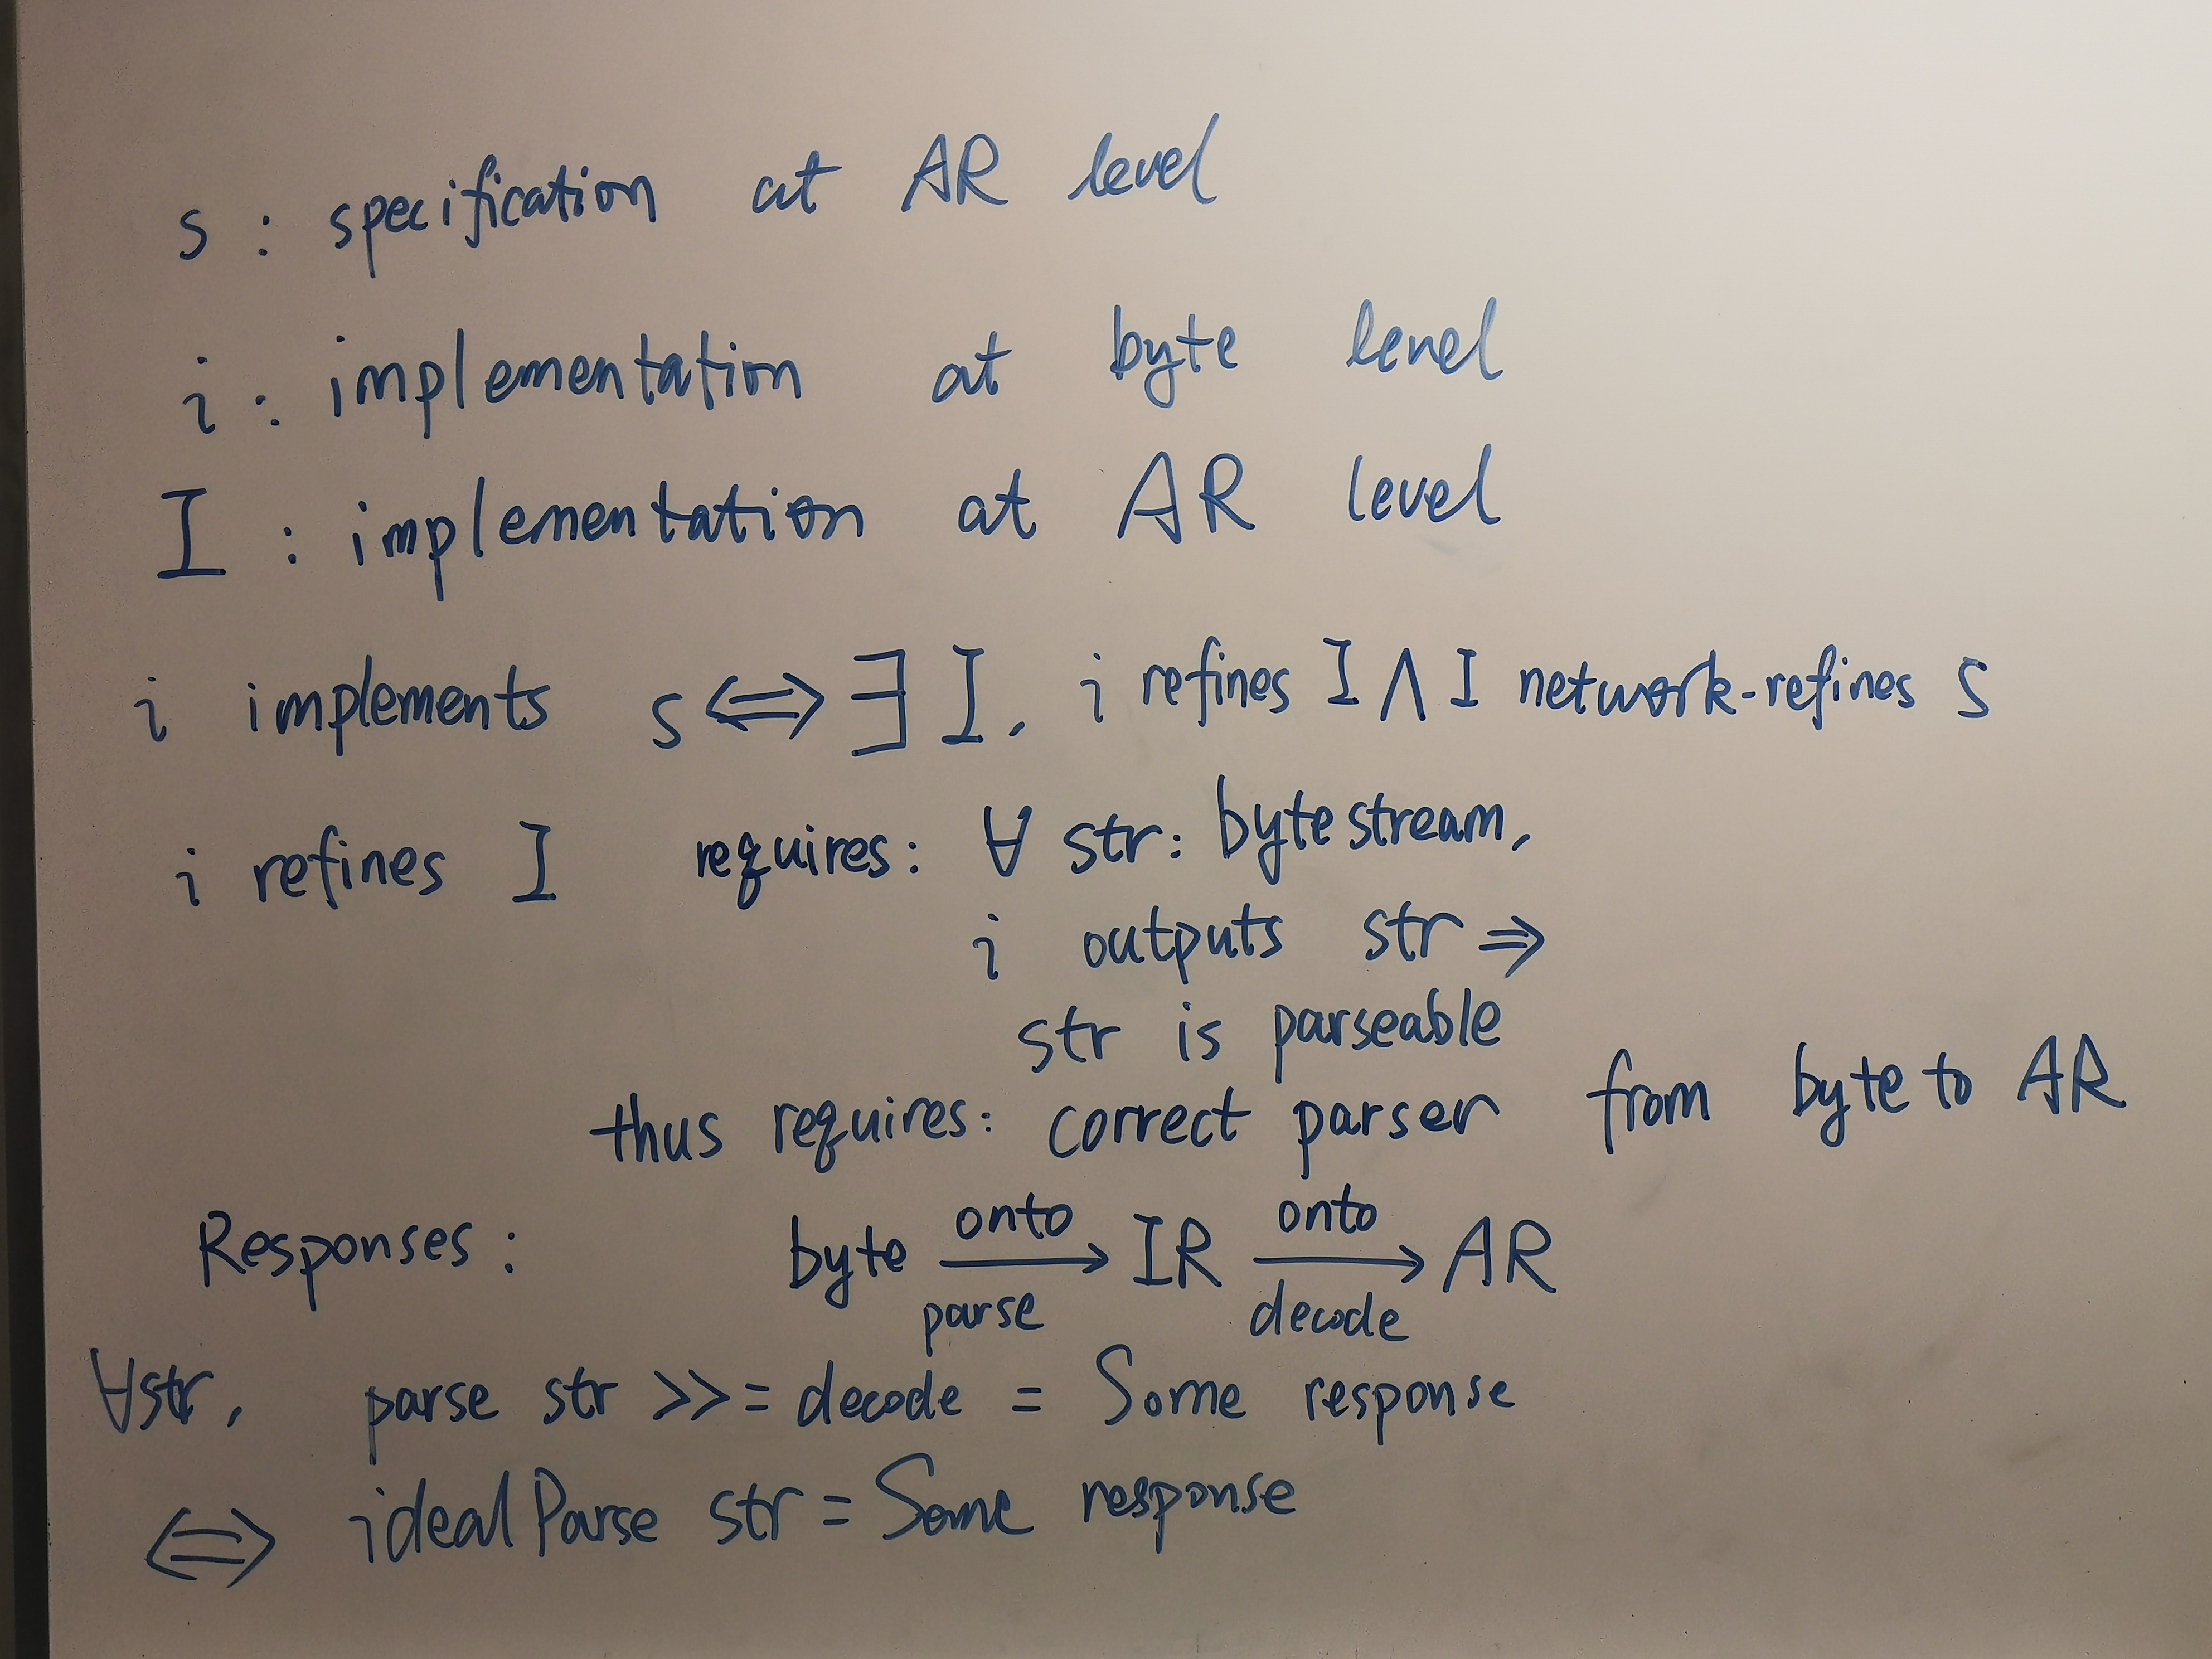
\includegraphics[width=\textwidth]{figures/ir-parse}
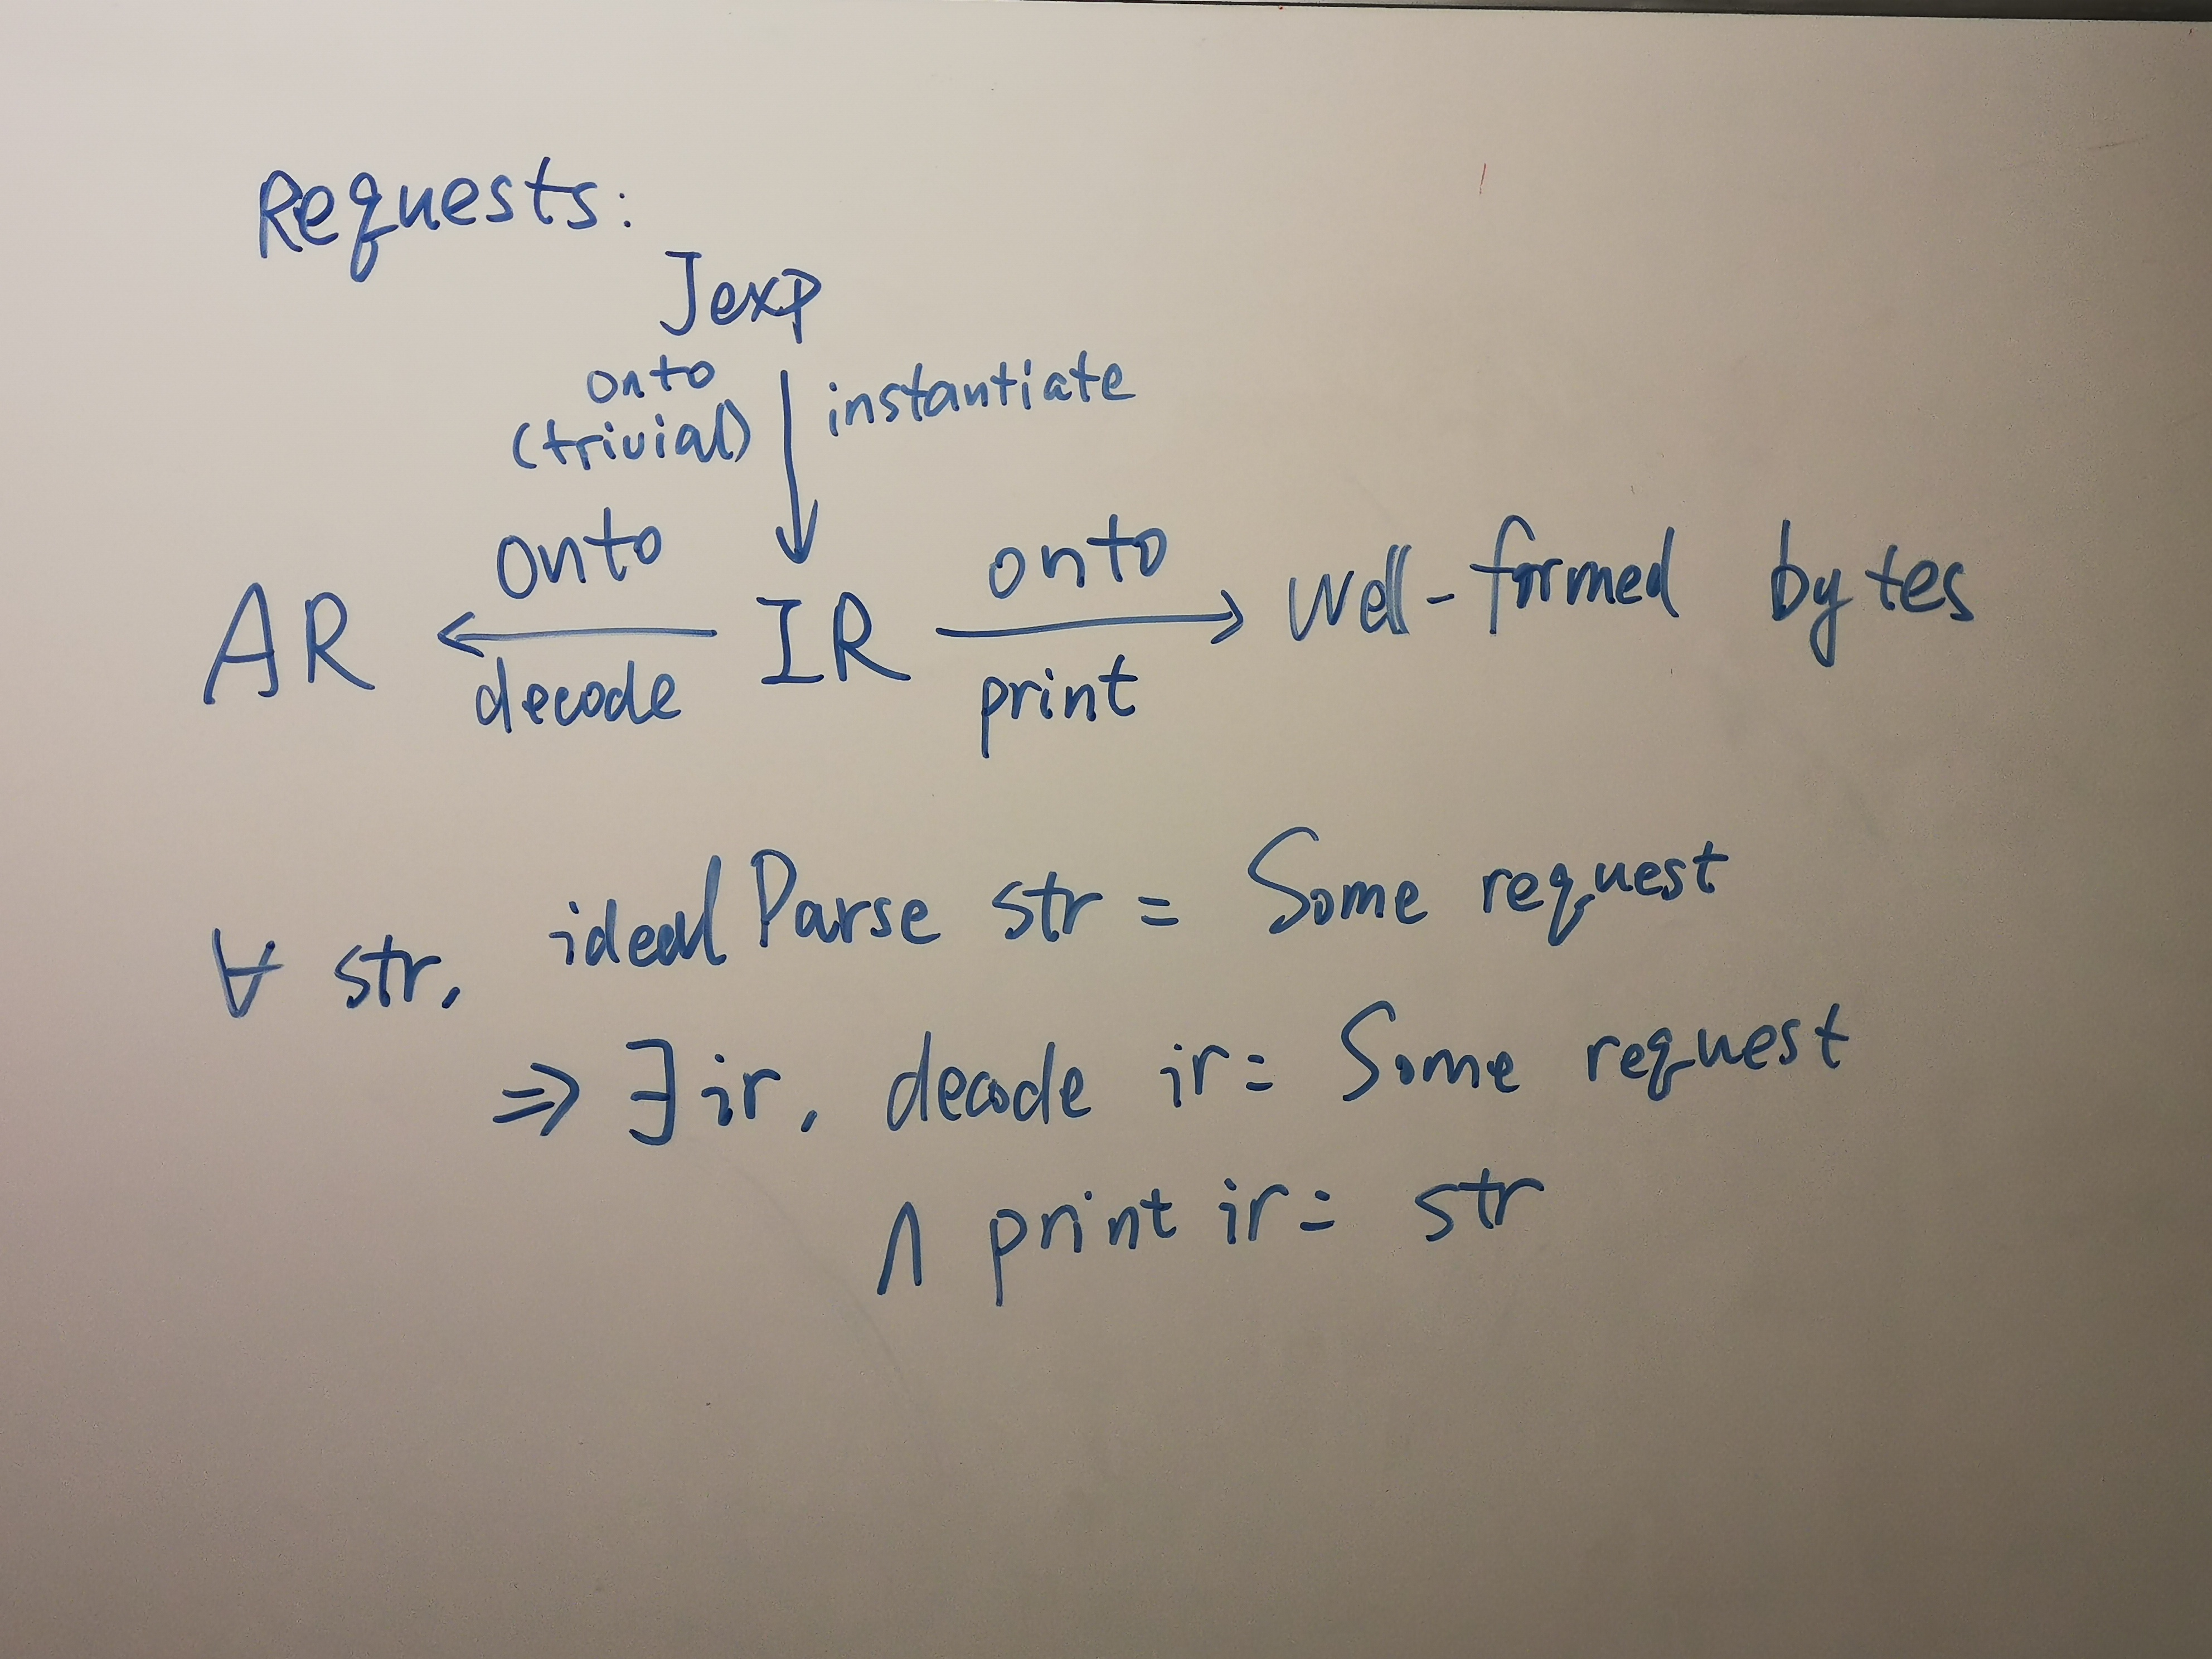
\includegraphics[width=\textwidth]{figures/ir-print}

\end{document}
